\chapter{Il Lavoro Svolto}
\label{ch:lavoro_svolto}
All'interno di questo capitolo è presente la descrizione delle cinque fasi di elaborazione del monitor real-time e del caso di studio riguardante il computer di bordo del velivolo F-16. Per ciascuna fase sono indicati i \textbf{dati in ingresso}, gli \textbf{strumenti utilizzati}, la \textbf{logica delle scelte progettuali} e i \textbf{risultati prodotti}, corredati da codice sorgente e schermate.

% ============================================================
\section{Fase 1 --- Architettura del Progetto e Build System}
\label{sec:fase1_build}
% ============================================================

\noindent\textbf{Dati in ingresso:} struttura del workspace di sviluppo.\\
\textbf{Strumenti utilizzati:} GNU Make, \texttt{gcc}/\texttt{g++}, \texttt{fastddsgen}.\\
\textbf{Risultati prodotti:} binari ELF in \texttt{bin/app/}, archivi statici \texttt{.a} in \texttt{bin/lib/}.

\bigskip

Prima di implementare le logiche di schedulazione Real-Time, è necessario costruire un'architettura del workspace in grado di gestire i vari componenti che costituiscono la struttura utilizzata. Questo progetto, che utilizza le librerie in linguaggio C, codice C++, middleware FastDDS, e script Python per l'analisi statistica, necessita che tutti gli elementi precedentemente citati debbano essere gestiti in modo ordinato e univoco.

\subsection{Struttura delle Directory}

La scelta fatta consiste nella \textbf{separazione tra sorgenti e artefatti} in due directory distinte: \texttt{src/} per il codice e \texttt{bin/} per i prodotti della compilazione. Questa scelta garantisce ordine e compattezza alla struttura del codice, permettendo allo sviluppatore di lavorare in un ambiente ottimizzato.

\subsubsection{La Directory dei Sorgenti (\texttt{src/})}

\begin{itemize}
	\item \textbf{\texttt{src/app/}:} Contiene i \textit{main()} di ogni processo eseguibile. Ogni applicazione ospita nella propria sottocartella un Makefile dedicato per l'aggiornamento del codice. Questa scelta permette di compilare un singolo applicativo senza scatenare la ricompilazione di tutti gli altri. Le applicazioni presenti sono:
	\begin{itemize}
		\item \texttt{F16\_Computer}: simulatore del computer di bordo.
		\item \texttt{Broadcastner} e \texttt{Listener}: nodi publisher e subscriber DDS per messaggi  \texttt{Geometric Point}.
		\item \texttt{ImageSender} e \texttt{ImageSubscriber}: scambio di immagini su rete DDS.
		\item \texttt{app10g}: esempio didattico con due task periodici su core dedicati.
	\end{itemize}
	
	\item \textbf{\texttt{src/lib/}:} Ospita tutte le librerie:
	\begin{itemize}
		\item \texttt{lib/}: Contiene \texttt{activity} (libreria principale dei task periodici), \texttt{time} (gestione del tempo), \texttt{trace} (iniezione marker nel kernel) e le librerie avioniche F-16. Questi moduli non hanno dipendenze da FastDDS e possono essere compilati ed eseguiti su qualsiasi sistema Linux.
		\item \texttt{dds\_lib/}: contiene un wrapper C++ sopra le API native di FastDDS. Questo perché creare un publisher richiede l'istanziazione di cinque oggetti separati (\texttt{DomainParticipant}, \texttt{Publisher}, \texttt{Topic}, \texttt{DataWriter}, \texttt{TypeSupport}). Il wrapper riduce tutto questo a una singola chiamata \texttt{start()}.
		\item \texttt{image\_lib/}: classi per la serializzazione di frame OpenCV in messaggi DDS \texttt{sensor\_msgs/Image}.
		\item \texttt{generated\_msg/}: codice generato automaticamente da \texttt{fastddsgen} dai file IDL. Il contenuto di questa cartella non viene mai modificato manualmente: è rigenerato ogni volta che cambia un file IDL.
	\end{itemize}
	
	\item \textbf{\texttt{src/msg/}:} File IDL che definiscono i protocolli di comunicazione DDS (\texttt{geometry\_msgs.idl}, \texttt{sensor\_msgs.idl}, \texttt{nav\_msgs.idl}). Questi file sono la definizione dei tipi di messaggio che le applicazioni DDS possono usare e quando bisogna modificarli e rieseguirli con \texttt{fastddsgen} essi  vengono rigenerati automaticamente e anche tutti i codici dedicati al loro utilizzo.
	
	\item \textbf{\texttt{src/tools/}:} Parser C++ (\texttt{thread\_analysis.cpp}) e monitor Python (\texttt{monitor.py}). Si trovano in \texttt{src/} poiché sono sorgenti da mantenere e nel caso aggiornare se ci fossero nuove modifiche da applicare.
\end{itemize}

\subsubsection{La Directory degli Artefatti (\texttt{bin/})}

\begin{itemize}
	\item \textbf{\texttt{bin/app/}:} Raccoglie tutti i binari in questo modo la ricerca dell'eseguibile alll'interno degli script bash che verranno usati (es. run trace.sh) 
	è sempre una singola operazione \texttt{find \$PROJECT\_ROOT/bin/app -name \$APP\_NAME}.
	\item \textbf{\texttt{bin/lib/}:} Raccoglie tutti gli archivi statici \texttt{.a}. Gli elementi presenti i questa cartella sono in modo  indipendente, quando compilate nelle rispettive direcotory di appartenenza, messe attraverso i loro makefile fisicamente in questa cartella.
	\item \textbf{\texttt{bin/tools/}:} Script bash che servono a fare il tracing dei vari eseguibili generati dai sorgenti rispettivi, verranno spiegati in modo più completo in questo punto \ref{bin/tools}
	\item \textbf{\texttt{bin/Test/}:} Vengono create delle cartelle dedicate per ongi simulazione con i risultati di ogni sessione di tracciamento. Ogni run genera una sottocartella con timestamp (es. \texttt{trace\_results\_app10g\_20260427\_212626/}), impedendo che esecuzioni successive sovrascrivano i risultati precedenti e permettendo il confronto storico tra sessioni.
\end{itemize}

\subsection{Build System: Architettura Decentralizzata dei Makefile}

\subsubsection{Perché Non un Makefile Unico?}

L'alternativa più semplice sarebbe un unico Makefile alla radice del progetto che gestisce ogni componente e quindi permette di aggiornare ogni componente all'interno del progetto in maniera immediata. Questa soluzione ha però tre problemi gravi per un progetto di questa complessità:

\begin{itemize}
	\item \textbf{Accoppiamento}: ogni modifica al Makefile centrale rischia di impattare la compilazione di componenti non correlati.
	\item \textbf{Scalabilità}: con 20+ componenti, un Makefile monolitico diventa ingestibile e difficile da debuggare.
	\item \textbf{Riusabilità}: è impossibile estrarre un singolo modulo e compilarlo in un altro progetto senza portarsi dietro l'intero Makefile.
\end{itemize}

Con l'architettura decentralizzata, ogni componente è autonomo: aggiungere un nuovo modulo significa creare una nuova directory con il proprio Makefile, senza toccare nulla di esistente.

\subsubsection{Perché il Linking Statico}

Il progetto utilizza esclusivamente librerie statiche \texttt{.a} invece di librerie condivise \texttt{.so}. Nei sistemi Real-Time, il linking dinamico introduce due forme di non-determinismo:
\begin{itemize}
	\item \textbf{Lazy binding}: alla prima chiamata di ogni funzione di libreria dinamica, il linker runtime deve risolvere l'indirizzo della funzione nella tabella PLT (\textit{Procedure Linkage Table}). Questo introduce una latenza variabile — tipicamente decine di microsecondi — alla prima invocazione, che può causare un picco di jitter al primo ciclo di ogni task.
	\item \textbf{Caricamento della libreria}: se una libreria condivisa viene scaricata dalla cache e deve essere ricaricata, il page fault risultante introduce una latenza imprevedibile.
\end{itemize}
Con il linking statico, tutto il codice è incorporato nel binario a tempo di compilazione. Al momento dell'esecuzione, non c'è nulla da risolvere o caricare dinamicamente: ogni chiamata a funzione è un salto diretto a un indirizzo già noto.

\subsubsection{Costruzione Locale e Linking Statico}

\begin{lstlisting}[language=make, caption={Makefile del nodo Listener: risoluzione path e dipendenze}]
	# Calcolo del percorso assoluto della root del progetto
	# partendo dalla posizione del Makefile stesso
	PROJECT_ROOT = $(abspath ../../../)
	BIN_DIR      = $(PROJECT_ROOT)/bin/app
	LIB_DIR      = $(PROJECT_ROOT)/bin/lib
	
	# Dipendenze esplicite: ogni libreria statica deve essere
	# compilata prima che questo target possa essere linkato
	LIBS_DEPS = $(LIB_DIR)/libActivity_library.a        \
	$(MSG_LIB_DIR)/libdds_communication.a    \
	$(wildcard $(MSG_LIB_DIR)/libdds_*.a)
\end{lstlisting}

Il costrutto \texttt{\$(abspath ../../../)} risolve il percorso relativo in percorso assoluto \textit{al momento della valutazione}. Questo è fondamentale: gli script bash invocano \texttt{make} da directory arbitrarie tramite la flag \texttt{-C}. Senza un percorso assoluto, i percorsi relativi sarebbero risolti rispetto alla directory corrente del processo chiamante, non rispetto alla posizione del Makefile.

La funzione \texttt{wildcard} per le librerie DDS cattura tutte le librerie generate da \texttt{fastddsgen}: ogni tipo di messaggio IDL produce una libreria separata (es. \texttt{libdds\_geometry\_msgs.a}, \texttt{libdds\_sensor\_msgs.a}), e il numero di queste librerie può variare quando si aggiungono nuovi tipi di messaggio.

\subsubsection{Gestione Dinamica delle Dipendenze degli Header}

Uno dei problemi classici dei build system è la gestione delle dipendenze dagli header: se si modifica \texttt{activity\_library.h} senza che Make lo sappia, il binario non viene ricompilato e incorpora una versione obsoleta della struttura.

\begin{lstlisting}[language=make, caption={Tracking automatico degli header per la ricompilazione}]
	# HDR_DEPS cattura tutti gli header che questo modulo include,
	# diretti o transitivi, attraverso le directory dichiarate
	HDR_DEPS = $(wildcard *.h) $(wildcard *.hpp)        \
	$(wildcard $(CORE_HDR)/*.h)              \
	$(wildcard $(DDS_HDR)/*.hpp)             \
	$(wildcard $(MSG_HDR)/*.h)
	
	# Il target dipende dal sorgente, dalle librerie E dagli header
	# Se uno qualsiasi di questi file e' piu' recente del binario,
	# Make lo ricompila automaticamente
	$(TARGET): Listener.cpp $(LIBS_DEPS) $(HDR_DEPS)
	@mkdir -p $(BIN_DIR)
	@echo ">>> Building $(TARGET)..."
	$(CXX) $(CXXFLAGS) $< -o $@ $(LDFLAGS)
\end{lstlisting}

Make confronta il timestamp di ogni prerequisito con il timestamp del target. Se almeno un prerequisito è più recente del binario, lo ricompila. Includendo tutti gli header come prerequisiti, si garantisce che qualsiasi modifica a un'interfaccia di libreria propaghi automaticamente la ricompilazione a tutti i moduli che la includono, senza necessità di \texttt{make clean}.

% \section{Fase 2 --- Librerie Core del Progetto}
\label{sec:fase2_librerie}
\label{ch:librerie_core}
% ============================================================

\noindent\textbf{Dati in ingresso:} file sorgente C/C++ in \texttt{src/lib/}.\\
\textbf{Risultati prodotti:} archivi statici \texttt{.a} in \texttt{bin/lib/}.

\bigskip

Le librerie mostrate in questo capitolo sono il fondamento su cui poggiano tutte le applicazioni. Ogni libreria ha un'unica funzione ben definita e non dipende da librerie di livello superiore. Questo permette di testare ogni componente in isolamento e di sostituirne uno senza impattare gli altri.

\subsection{Libreria \texttt{time}: Gestione del Tempo Monotónico POSIX}
\label{sec:lib_time}

\noindent\textbf{Posizione nel progetto:}
\begin{itemize}
	\item Interfaccia: \texttt{src/lib/lib/time/include/time\_library.h}
	\item Implementazione: \texttt{src/lib/lib/time/src/time\_library.c}
\end{itemize}

La libreria \texttt{time} risolve due problemi sottili che, se ignorati, portano a comportamenti non deterministici alll' interno dei sistemi Real-Time.

\subsubsection{Perché \texttt{CLOCK\_MONOTONIC} e non \texttt{CLOCK\_REALTIME}}

Esistono due modalità per gestire il tempo in Linux:
\begin{itemize}
	\item \textbf{\texttt{CLOCK\_REALTIME}}: Può essere modificato in qualsiasi momento e quindi se suncorregge un disallineamento di 200 ms mentre un task periodico dorme, il task interessato si sveglierà 200 ms prima del previsto, violando il suo periodo rompendo così uno dei vincoli dei sistemi Real-Time.
	\item \textbf{\texttt{CLOCK\_MONOTONIC}}: garantisce che il tempo venga gestito in modo che non possa essere modificato da nessuno in questo modo si garantisce come sorgente sicura per sistemi RT, permettendo di misurare intervalli precisi indipendentemente dal tempo assoluto del sistema.
\end{itemize}

La scelta di \texttt{CLOCK\_MONOTONIC} è quindi obbligata per garantire la correttezza della schedulazione periodica in scenari in cui il controllo dei vincoli temporali è critico.

\subsection{Libreria \texttt{trace}: Iniezione dei Marker nel Kernel}
\label{sec:lib_trace}

\noindent\textbf{Posizione nel progetto:}
\begin{itemize}
	\item Interfacce: \texttt{src/lib/lib/trace/include/trace\_marker.h} (e \texttt{marker.h})
	\item Implementazione: \texttt{src/lib/lib/trace/src/trace\_marker.c}
\end{itemize}

La libreria \texttt{trace} serve per avere un'interfaccia tra lo spazio utente dell'applicazione e il sottosistema \texttt{ftrace} del kernel Linux. Il suo scopo è permettere di avere dei marker temporali coincidenti con eventi di scheduling del kernel, i quali hanno come principale funzionalità il facilitare la lettura degli eventi che si verificano durante la simualzione.

\subsubsection{Perché scrivere i marker nel Kernel e non in un File Utente}

Un'alternativa più semplice sarebbe scrivere i marker in un file di log in spazio utente (es. con \texttt{fprintf} su un file). Questa soluzione ha però tre limitazioni critiche:
\begin{itemize}
	\item \textbf{Mancanza di sincronizzazione}: il timestamp del marker sarebbe quello del processo utente che può differire dal timestamp del kernel di decine di microsecondi a causa dei context switch che ci potrebbero essere.
	\item \textbf{Overhead elevato}: \texttt{fprintf} su file comporta lock, buffering e potenziali system call bloccanti.
\end{itemize}

Il file \texttt{/sys/kernel/debug/tracing/trace\_marker}
 (o \texttt{/sys/kernel/tracing/trace\_marker} in sistemi più recenti)
  risolve tutti questi problemi: la scrittura viene eseguita direttamente nel buffer del kernel con il timestamp del kernel, garantendo un perfetto allineamento temporale con tutti gli eventi critici di sistema, come \texttt{sched\_switch} e \texttt{sched\_wakeup}.

\subsubsection{Due Versioni: con Stato e Inline}

La scelta di offrire due implementazioni risponde a esigenze diverse.
La versione con stato (\texttt{trace\_marker.h/c}) mantiene un file descriptor globale ed è preferibile per applicazioni che scrivono milioni di marker (come i task periodici con periodo di 10 ms): il file descriptor viene aperto una sola volta chiamando la \texttt{init\_tracing()} e riutilizzato in modo sicuro per le performance e gestendone la chiusura con \texttt{close\_tracing()}. 

La versione inline (nell'header aggiuntivo \texttt{marker.h}) utilizza invece una variabile locale statica avendo un' apertura alla prima chiamata. Questo risulta comodo per test semplici dove vengono testati pochi thread.


\subsection{Libreria \texttt{activity}: Struttura del Task Periodico}
\label{sec:lib_activity}

\noindent\textbf{Posizione nel progetto:}
\begin{itemize}
	\item Interfaccia: \texttt{src/lib/lib/activity/include/activity\_library.h}
	\item Implementazione: \texttt{src/lib/lib/activity/src/activity\_library.c}
\end{itemize}

La libreria \texttt{activity} è il componente più importante. Il suo obiettivo è fornire l'implementazione completa di un task periodico Real-Time, nascondendo allo sviluppatore tutta la complessità nella gestione di scrittura dei marker e di implementazione della periodic task dove l'implementazione viene trattata in questo punto \ref{activity_library}.

\subsubsection{Il Problema del Drift Cumulativo e la sua Soluzione}

Il modo più semplice di implementare un task periodico è usare uno sleep relativo come \texttt{usleep(periodo\_in\_microsecondi)}. Tuttavia, questo approccio è profondamente errato. Se il task impiega $t_{exec}$ ms, il prossimo risveglio sarà a $t_{start} + t_{exec} + T_{sleep}$, non a $t_{start} + T_{periodo}$. Andando avanti la simulazione accumula questi ritardi e i tasks perdono la sincronizzazione con il tempo reale (fenomeno del \textit{drift cumulativo}). 
La libreria \texttt{activity} risolve questo problema con l'utilizzo di \texttt{clock\_nanosleep} combinata al flag \texttt{TIMER\_ABSTIME}, è proprio in questo modo che il \texttt{PeriodicTask} acquisisce il tempo corrente all'inizio, e in ogni ciclo calcola in anticipo l'istante assoluto in cui risvegliarsi ignorando totalmente quanto tempo sia stato effettivamente speso in esecuzione. 

\paragraph{Utilizzo dei marker da parte del parser.} All'interno del ciclo, \texttt{PeriodicTask} chiama \texttt{write\_trace\_marker} cinque volte per delimitare il periodo. Questi marker generano una sequenza di eventi nel log del kernel che il parser C++ usa per estrarre le metriche:
\begin{itemize}
	\item \textbf{\texttt{PERIOD\_START} $\to$ \texttt{PERIOD\_START} successivo}: periodo reale misurato. Confrontato con il periodo scelto per calcolare il Jitter.
	\item \textbf{\texttt{FUNCTION\_START} $\to$ \texttt{FUNCTION\_END}}: misurazione del WCET e ACET della funzione applicativa, isolata dalle attese.
	\item \textbf{\texttt{PERIOD\_START} $\to$ \texttt{FUNCTION\_END}}: Response Time, che include eventuali periodi di prelazione o interferenze subite prima che il task ottenesse realmente la CPU.
	\item \textbf{\texttt{FUNCTION\_END} $\to$ \texttt{PERIOD\_END}}: Slack Time, ovvero il tempo rimanente speso a dormire prima della scadenza della deadline o inizio del nuovo periodo.
\end{itemize}

\subsubsection{La Funzione di Carico Computazionale: \texttt{activity\_load}}

Questa libreria espone anche la funzione \texttt{activity\_load}, il cui scopo è generare un carico computazionale che serve a simulare il reale sforzo di una CPU in un contesto realistico. 

\paragraph{Perché \texttt{volatile}:} il metodo si basa su un ciclo for che calcola il risultato di operazioni matematiche assegnando alla variabile \texttt{result} il risultato. Senza la keyword \texttt{volatile}, il compilatore moderno (gcc/g++) analizzerebbe il ciclo, concluderebbe che \texttt{result} non viene mai letto o restituito all'esterno, e \textbf{eliminerebbe completamente l'intero loop} provocando la mancata visione all'interno del monitor dell'effettiva esecuzione della periodic task. La keyword \texttt{volatile} indica al compilatore che il valore potrebbe essere letto da entità esterne  impedendo così in modo rigoroso qualsiasi ottimizzazione del ciclo.

\paragraph{Perché operazioni trigonometriche.}  Il parametro \texttt{cost} permette di calibrare il carico computazionale, ogni unità corrisponde a $10^6$ iterazioni, dando in questo modo allo sviluppatore la possibilità di modificare agevolmente lo sforzo computazionale della propria periodic task.


\subsection{Libreria \texttt{dds\_lib}: Wrapper al Middleware FastDDS}

Questa astrazione si compone in due parti: il modulo Publisher (Broadcastner) e il modulo Subscriber (Listener).

\subsubsection{Modulo \texttt{Broadcastner}}
\label{sec:lib_broadcastner}

\noindent\textbf{Posizione nel progetto:}
\begin{itemize}
	\item Interfaccia: \texttt{src/lib/dds\_lib/broadcastner/include/Broadcastner.hpp}
	\item Implementazione: \texttt{src/lib/dds\_lib/broadcastner/src/Broadcastner.cpp}
\end{itemize}

\paragraph{Implementazione:}
Per creare il Broadcastner per creare  un \texttt{DomainParticipant} è stato implementato un \texttt{DomainParticipantFactory} per poi registrare il \texttt{TypeSupport} e creare un \texttt{Publisher} che comunica su un \texttt{Topic} e infine la creazione di un \texttt{DataWriter}. Ognuno di questi passi richiede la gestione dei parametri QoS (\textit{Quality of Service}) fondamentali per la comunciazione in ambiente DDS. Senza il wrapper, ogni applicazione che vuole pubblicare dati dovrebbe ripetere e manutenere questa ingombrante sequenza di decine di righe di codice. Il wrapper \texttt{Broadcastner} incapsula l'intera complessità in due semplici metodi: un \texttt{start()} che prende il tipo di messaggio, topic e dominio configurando tutto, e un \texttt{publish()} che casta e invia il payload DDS in modo astratto. Internamente, il metodo \texttt{start} configura anche il \texttt{PubListener}, un listener interno che intercetta in modo trasparente gli eventi asincroni come \texttt{on\_publication\_matched}. Questo permette di stampare a terminale log essenziali quando un subscriber si connette o si disconnette dal topic, un aspetto fondamentale per il debugging e la validazione della fase di discovery della rete distribuita.
\clearpage
\subsubsection{Modulo \texttt{Listener}}
\label{sec:lib_listener}

\noindent\textbf{Posizione nel progetto:}
\begin{itemize}
	\item Interfaccia: \texttt{src/lib/dds\_lib/listener/include/Listener.hpp}
	\item Implementazione: \texttt{src/lib/dds\_lib/listener/src/Listener.cpp}
\end{itemize}

Il modulo \texttt{Listener} implementa il lato subscriber in ricezione. A differenza di molti approcci, la sua architettura è puramente event-driven: invece di fare un polling attivo ed estenuante per verificare se sono arrivati nuovi messaggi (il che consumerebbe CPU inutilmente distruggendo l'efficienza RT del sistema), è il middleware DDS stesso a chiamare automaticamente il callback di callback del metodo \texttt{on\_data\_available()} ogni volta che un messaggio utile viene consegnato.

Ed è all'interno di questo metodo che sono stati iniettati i kernel marker: ciò consente di individuare con assoluta precisione, nel file di trace, l'istante in cui il Listener riceve e notifica un messaggio sulla rete DDS. Il \texttt{Listener} a sua volta incapsula la creazione e la registrazione sicura del \texttt{DomainParticipant}, \texttt{Subscriber} e \texttt{DataReader}.



\subsection{Libreria \texttt{generated\_msg}: Classi di Messaggistica DDS}
\label{sec:lib_generated_msg}

\noindent\textbf{Posizione nel progetto:}
\begin{itemize}
	\item Destinazione generati: \texttt{src/lib/generated\_msg/}
	\item IDL in ingresso: \texttt{src/msg/}
\end{itemize}

La sottocartella \texttt{generated\_msg} è il punto di intersezione tra le definizioni formali e neutrali dei messaggi (file IDL, \textit{Interface Definition Language}) e il codice C++ direttamente utilizzabile dalle applicazioni.

\subsubsection{Il Processo di Generazione}

La compilazione esegue il tool \texttt{fastddsgen} (fornito dal framework) che legge in automatico ogni file IDL e produce le implementazioni C++, generando:
\begin{itemize}
	\item \textbf{La struttura dati del messaggio}: per ogni campo definito nell'IDL (es. \texttt{float64 x; float64 y; float64 z;} per un \texttt{Point}), viene tradotto in una classe C++ nativa completa di getter, setter fortemente tipizzati e operatori di assegnamento.
	\item \textbf{La serializzazione CDR}: metodi ottimizzati come \texttt{serialize()} e \texttt{deserialize()} che si preoccupano di impacchettare in bytes la struttura in formato CDR (\textit{Common Data Representation}), lo standard dell'Object Management Group (OMG). Il CDR è vitale in quanto garantisce l'interoperabilità di rete assoluta tra nodi in architetture hardware o OS profondamente diversi (assicurando l'integrità fra macchine little-endian e big-endian).
	\item \textbf{Il TypeSupport}: come la classe \texttt{XxxPubSubType}, che registra formalmente il nuovo tipo custom nel middleware DDS e fornisce tutte le funzioni di supporto hash necessarie per la discovery logica e il matching rapido tra publisher e subscriber sulla rete.
\end{itemize}

\clearpage

\subsection{Libreria \texttt{math}: Funzioni Algebriche Ausiliarie}
\label{sec:lib_math}

\noindent\textbf{Posizione nel progetto:}
\begin{itemize}
	\item Interfaccia: \texttt{src/lib/lib/math/include/math\_library.h}
	\item Implementazione: \texttt{src/lib/lib/math/src/math\_library.c}
\end{itemize}

La libreria \texttt{math} è una libreria di supporto minimale che implementa operazioni aritmetiche banali come il recupero della somma e del valore massimo dagli elementi di un array di interi.

Queste funzioni sono usate principalmente negli applicativi di test ed entry point per calcolare metriche aggregate come le somme di carichi computazionali richiesti o per trovare i picchi massimi tra le iterazioni, evitando ogni volta la reimplementazione di logiche simili e l'inclusione di pesanti macro framework. 
La loro esistenza come libreria C pura e separata — anziché come funzioni inline ingombranti all'interno dei file \texttt{.c} applicativi — è motivata dalla ferrea volontà architetturale di mantenere ogni file sorgente focalizzato solo ed unicamente sulla propria responsabilità principale, in questo modo, i file che definiscono le applicazioni RT descrivono solo la complessa logica di scheduling e la composizione delle activity, ma non come eseguire algoritmi matematici sui dati di configurazione.



% ============================================================
\section{Fase 3 --- Le Applicazioni del Progetto}
\label{sec:fase3_applicazioni}
% ============================================================

\noindent\textbf{Dati in ingresso:} librerie core compilate in \texttt{bin/lib/}.\\
\textbf{Strumenti utilizzati:} primitive POSIX, middleware FastDDS, OpenCV.\\
\textbf{Risultati prodotti:} binari in \texttt{bin/app/} pronti per il tracciamento.

% ============================================================
\subsection{Applicazione \texttt{app10g}: Due Task su Core Distinti}
\label{cap:app10g_esempio}
% ============================================================

L'applicazione \texttt{app10g} (\texttt{src/app/app10g/app10g.c}) è l'esempio didattico di
riferimento: due task periodici su core dedicati, senza alcuna interferenza da prelazione.
Il codice viene mostrato e interrotto nei punti  rilevanti per evidenziare il funzionamento del codice ed il perché delle scelte di progetto.

% ============================================================
\subsubsection{Dipendenze e Gestione degli Errori:}
% ============================================================

Il file apre con la direttiva \texttt{\_GNU\_SOURCE}, indispensabile per sbloccare le
estensioni GNU/POSIX non standard (tra cui \texttt{pthread\_setname\_np} e
\texttt{pthread\_attr\_setaffinity\_np}), e include i tre header del progetto:
\texttt{time\_library.h} (gestione del tempo POSIX), \texttt{trace\_marker.h} (scrittura
su \texttt{ftrace}) e \texttt{activity\_library.h} (struttura dati e task periodico).

\begin{lstlisting}[language=C, caption={\texttt{app10g.c} -- direttive e include}]
	#define _GNU_SOURCE
	#include <errno.h>
	#include <math.h>
	#include <pthread.h>
	#include <sched.h>
	#include <stdbool.h>
	#include <stdint.h>
	#include <stdio.h>
	#include <stdlib.h>
	#include <string.h>
	#include <time.h>
	
	#include "time_library.h"
	#include "trace_marker.h"
	#include "activity_library.h"
\end{lstlisting}

La macro \texttt{handle\_error} incapsula il pattern standard di gestione degli errori
POSIX: se il codice di ritorno è diverso da zero, imposta \texttt{errno}, stampa il
messaggio su \texttt{stderr} tramite \texttt{perror} e termina il processo con
\texttt{EXIT\_FAILURE}.

\begin{lstlisting}[language=C, caption={\texttt{app10g.c} -- macro di gestione errori}]
	#define handle_error(en, msg)                                                  \
	if (en != 0) {                                                               \
		errno = en;                                                                \
		perror(msg);                                                               \
		exit(EXIT_FAILURE);                                                        \
	}
\end{lstlisting}

% ============================================================
\subsubsection{Inizializzazione del Tracing e Dichiarazione delle Variabili}
% ============================================================

All'ingresso del \texttt{main}, la prima operazione è \texttt{init\_tracing()}: apre il
file descriptor verso \texttt{/sys/kernel/debug/tracing/trace\_marker} (o il percorso
alternativo \texttt{/sys/kernel/tracing/trace\_marker} su kernel più recenti). Questo file
è il canale privilegiato attraverso cui il codice utente inietta eventi nel ring buffer del
kernel, rendendoli visibili a \texttt{trace-cmd} e KernelShark.

\begin{lstlisting}[language=C, caption={\texttt{app10g.c} -- apertura del tracing e variabili}]
	int main(int argc, char *argv[]) {
		// Inizializza il file descriptor per i marker di tracciamento
		init_tracing();
		
		// Setup per i thread 1 e 2
		pthread_t thread1, thread2;
		pthread_attr_t attr1, attr2;
		struct sched_param param1, param2;
		int ret_err;
		
		// Definiamo due maschere diverse per i core
		cpu_set_t cpuset_core1;
		cpu_set_t cpuset_core2;
	\end{lstlisting}
	
	Le strutture \texttt{pthread\_attr\_t} conterranno tutta la configurazione del thread prima
	della creazione; \texttt{struct sched\_param} trasporta la priorità RT; \texttt{cpu\_set\_t}
	è la maschera di affinità CPU, un bitmask in cui ogni bit corrisponde a un core logico.
	
	% ============================================================
	\subsubsection{Inizializzazione degli Attributi e Policy RT}
	% ============================================================
	
	I due oggetti attributo vengono inizializzati con \texttt{pthread\_attr\_init} e
	immediatamente configurati con la policy \texttt{SCHED\_FIFO}.
	Il flag \texttt{PTHREAD\_EXPLICIT\_SCHED} è cruciale: senza di esso il figlio
	erediterebbe la policy \texttt{SCHED\_OTHER}  del processo padre, non permettendo la configurazione real-time.
	
	\begin{lstlisting}[language=C, caption={\texttt{app10g.c} -- init attributi e policy SCHED\_FIFO}]
		pthread_attr_init(&attr1);
		pthread_attr_init(&attr2);
		
		// Impostazione della policy SCHED_FIFO (Real-Time) per entrambi
		pthread_attr_setinheritsched(&attr1, PTHREAD_EXPLICIT_SCHED);
		pthread_attr_setschedpolicy(&attr1, SCHED_FIFO);
		
		pthread_attr_setinheritsched(&attr2, PTHREAD_EXPLICIT_SCHED);
		pthread_attr_setschedpolicy(&attr2, SCHED_FIFO);
	\end{lstlisting}
	
	Con \texttt{SCHED\_FIFO}, lo scheduler Linux ( assegna la CPU
	al thread con la priorità più alta tra quelli pronti; un thread RT non viene mai prelazionato da thread a priorità inferiore se si usa come algoritmo di schedulazione RM(Rate Monotonic).
	% ============================================================
	\subsubsection{Affinità di Core}
	% ============================================================
	
	La sezione seguente vincola ogni thread a un core fisico, per permettere di testare varie simulazione in cui si cambiano i core fisici su cui i thread girano effetivamente, distinto tramite la	maschera \texttt{cpu\_set\_t}.
	\texttt{CPU\_ZERO} azzera la maschera, \texttt{CPU\_SET(n, ...)} imposta il bit
	corrispondente al core $n$, e \texttt{pthread\_attr\_setaffinity\_np} registra la
	maschera nell'attributo del thread.
	
	\begin{lstlisting}[language=C, caption={\texttt{app10g.c} -- affinità di core}]
		// ==========================================
		// CONFIGURAZIONE AFFINITA' CORE
		// ==========================================
		
		// Set per il Thread 1 -> CORE 1
		CPU_ZERO(&cpuset_core1);
		CPU_SET(1, &cpuset_core1);
		pthread_attr_setaffinity_np(&attr1, sizeof(cpu_set_t), &cpuset_core1);
		
		// Set per il Thread 2 -> CORE 2
		CPU_ZERO(&cpuset_core2);
		CPU_SET(2, &cpuset_core2);
		pthread_attr_setaffinity_np(&attr2, sizeof(cpu_set_t), &cpuset_core2);
	\end{lstlisting}
	
	L'isolamento su core distinti garantisce che i due task non si contendano mai la
	stessa risorsa hardware, nulla vieta di modificare il codice in modo da vedere come va la simulazione nel caso di prelazione reciproca.
	% ============================================================
	\subsubsection{Configurazione dei Thread}
	% ============================================================
	
	Ogni thread viene descritto da una struttura \texttt{t\_activity\_par} che aggrega
	nome, funzione di carico, periodo, parametro e deadline.
	La priorità Rate Monotonic viene calcolata come $99 - \lfloor T/10 \rfloor$, poi
	saturata a 1 per evitare valori non validi.
	
	\begin{lstlisting}[language=C, caption={\texttt{app10g.c} -- Thread 1: Core 1, periodo 1000 ms}]
		// ==========================================
		// -- THREAD 1 -- (Core 1)
		// ==========================================
		t_activity_par activity_1;
		snprintf(activity_1.name, 15, "Activity_1");
		activity_1.function  = activity_load; // Funzione importata dalla libreria
		activity_1.period    = 1000;
		activity_1.parameter = 10;
		activity_1.deadline  = 1000;
		
		param1.sched_priority = 99 - (activity_1.period / 10); // = 1 (saturato)
		if (param1.sched_priority < 1) param1.sched_priority = 1;
		pthread_attr_setschedparam(&attr1, &param1);
		
		ret_err = pthread_create(&thread1, &attr1, PeriodicTask, (void *)&activity_1);
		handle_error(ret_err, "Error in creating PeriodicTask 1");
		pthread_setname_np(thread1, "Activity_1");
	\end{lstlisting}
	
	\begin{lstlisting}[language=C, caption={\texttt{app10g.c} -- Thread 2: Core 2, periodo 1200 ms}]
		// ==========================================
		// -- THREAD 2 -- (Core 2)
		// ==========================================
		t_activity_par activity_2;
		snprintf(activity_2.name, 15, "Activity_2");
		activity_2.function  = activity_load; // Funzione importata dalla libreria
		activity_2.period    = 1200;
		activity_2.parameter = 20;
		activity_2.deadline  = 1200;
		
		param2.sched_priority = 99 - (activity_2.period / 10);
		if (param2.sched_priority < 1) param2.sched_priority = 1;
		pthread_attr_setschedparam(&attr2, &param2);
		
		ret_err = pthread_create(&thread2, &attr2, PeriodicTask, (void *)&activity_2);
		handle_error(ret_err, "Error in creating PeriodicTask 2");
		pthread_setname_np(thread2, "Activity_2");
	\end{lstlisting}
	
	Il nome assegnato con \texttt{pthread\_setname\_np} (massimo 15 caratteri, limite
	imposto dal kernel) è quello che appare direttamente in KernelShark e nell'output
	di \texttt{trace-cmd report}, permettendo di identificare immediatamente il task
	responsabile di ogni evento nel ring buffer.
	
	% ============================================================
	\subsubsection{Cleanup e Attesa}
	% ============================================================
	
	Una volta creati i thread, gli oggetti attributo non servono più: vengono distrutti
	per liberare le risorse interne allocate da \texttt{pthread\_attr\_init}.
	Il \texttt{main} si blocca poi sulle due \texttt{pthread\_join}, che in un sistema
	embedded reale non ritorneranno mai (i task girano all'infinito nel loro loop
	\texttt{while(1)}); tuttavia la chiamata è necessaria per impedire che il processo
	termini immediatamente.
	Prima di uscire, \texttt{close\_tracing()} chiude il file descriptor verso
	\texttt{trace\_marker}, assicurando che tutti i byte in sospeso vengano svuotati.
	
	\begin{lstlisting}[language=C, caption={\texttt{app10g.c} -- pulizia e join}]
		// Pulizia attributi
		pthread_attr_destroy(&attr1);
		pthread_attr_destroy(&attr2);
		
		// Attesa completamento (in un sistema reale girano all'infinito)
		pthread_join(thread1, NULL);
		pthread_join(thread2, NULL);
		
		// Chiude il file descriptor dei marker
		close_tracing();
		
		exit(0);
	}
\end{lstlisting}

% ============================================================
\subsubsection{Caratteristiche Rilevanti}
% ============================================================

\begin{itemize}
	\item \textbf{core distinti:} i due task non condividono mai la stessa risorsa hardware; la maschera di affinità garantisce che il kernel non migri mai il thread verso un core diverso.
	\item \textbf{Carico differenziato:} la variabile parameter attraverso la funzione \texttt{activity\_load}, permette di osservare tempi di esecuzione differenti nelle tracce, infatti il parametro decide all'interno della funzione quanti cicli di CPU vengono impiegati producendo effetti diversi.
	\item \textbf{Tracciamento automatico:} l'instrumentazione completa (4 marker per periodo: \texttt{PERIOD\_START}, \texttt{FUNCTION\_START}, \texttt{FUNCTION\_END}, \texttt{SLEEP\_START}/\texttt{PERIOD\_END}) è interamente delegata a \texttt{PeriodicTask}, rendendo \texttt{app10g.c} libero da codice di tracing.
\end{itemize}



\subsubsection{\texttt{PeriodicTask eseguita dall' applicazione:}}
\label{activity_library}
% ============================================================

\texttt{PeriodicTask} è la funzione eseguita da ogni thread.
Segue lo schema classico del task periodico POSIX: campiona il tempo assoluto iniziale con \texttt{CLOCK\_MONOTONIC}, poi entra in un loop infinito che:

\begin{enumerate}
	\item Scrive il marker \texttt{PERIOD\_START\_<name>} nel ring buffer del kernel.
	\item Calcola il prossimo istante di rilascio aggiungendo il periodo al tempo corrente.
	\item Scrive il marker \texttt{FUNCTION\_START\_<name>} e avvia la misurazione del tempo.
	\item Esegue la funzione di carico (con la firma corretta).
	\item Scrive il marker \texttt{FUNCTION\_END\_<name>}.
	\item Scrive il marker \texttt{SLEEP\_START\_<name>} e si sospende con \texttt{clock\_nanosleep} in modalità \texttt{TIMER\_ABSTIME}.
	\item Alla ripresa scrive \texttt{PERIOD\_END\_<name>} e ricomincia.
\end{enumerate}

Iniziamo analizzando la fase di setup del task, dove vengono preparate le variabili per la temporizzazione e per la generazione dei marker nel kernel:

\begin{lstlisting}[language=C, caption={\texttt{activity\_library.c} -- Inizializzazione di \texttt{PeriodicTask}}]
	/*
	* activity_library.c
	*/
	#include "activity_library.h"
	#include "trace_marker.h"
	#include <math.h>
	#include <stdio.h>
	
	void *PeriodicTask(void *ptr) {
		t_activity_par activity;
		activity = *((t_activity_par *)ptr);
		
		struct timespec exec_release_time;
		uint64_t exec_start_time;
		uint64_t exec_end_time;
		char marker[128];
		
		// BASELINE: acquisisce il tempo corrente come riferimento assoluto
		clock_gettime(CLOCK_MONOTONIC, &exec_release_time);
	\end{lstlisting}
	
	A questo punto inizia il ciclo infinito. L'uso di \texttt{TIMER\_ABSTIME} in \texttt{clock\_nanosleep} è fondamentale per la
	correttezza temporale: il thread si sveglia all'istante assoluto $t_0 + k \cdot T$,
	indipendentemente da quanto tempo ha impiegato la funzione di carico.
	Un'attesa relativa (\texttt{TIMER\_RELTIME}) accumulerebbe invece l'errore di ogni
	iterazione, causando una deriva del periodo nel tempo.
	
	\begin{lstlisting}[language=C, caption={\texttt{activity\_library.c} -- Ciclo infinito di \texttt{PeriodicTask}}]
		while (1) {
			snprintf(marker, sizeof(marker), "PERIOD_START_%s", activity.name);
			write_trace_marker(marker);
			
			// CALCOLO PREVENTIVO del prossimo rilascio
			time_add_millisecs(&exec_release_time, activity.period);
			
			snprintf(marker, sizeof(marker), "FUNCTION_START_%s", activity.name);
			write_trace_marker(marker);
			
			exec_start_time = time_current_millisecs();
		\end{lstlisting}
		
		Il blocco successivo esegue l'effettivo carico computazionale. Per garantire la compatibilità con le diverse funzioni utente, il codice esegue un controllo sul puntatore a funzione:
		
		\begin{lstlisting}[language=C, caption={\texttt{activity\_library.c} -- Esecuzione carico e chiusura periodo}]
			// Chiamata con entrambi i parametri per compatibilita
			if (activity.function == (void (*)(void *, int))activity_load) {
				void (*func_single)(int) = (void (*)(int))activity.function;
				func_single(activity.parameter);
			} else {
				activity.function(activity.instance, activity.parameter);
			}
			
			exec_end_time = time_current_millisecs();
			
			snprintf(marker, sizeof(marker), "FUNCTION_END_%s", activity.name);
			write_trace_marker(marker);
			
			snprintf(marker, sizeof(marker), "SLEEP_START_%s", activity.name);
			write_trace_marker(marker);
			
			// BLOCCO ASSOLUTO anti-deriva
			clock_nanosleep(CLOCK_MONOTONIC, TIMER_ABSTIME, &exec_release_time, NULL);
			
			snprintf(marker, sizeof(marker), "PERIOD_END_%s", activity.name);
			write_trace_marker(marker);
		}
		
		pthread_exit((void *)ptr);
	}
\end{lstlisting}

\subsubsection{\texttt{activity\_load}: }
% ============================================================

\texttt{activity\_load} genera un carico computazionale controllato attraverso un
ciclo di operazioni floating-point (\texttt{sin}, \texttt{cos}, \texttt{tan}) su
\texttt{cost} milioni di iterazioni.

\begin{lstlisting}[language=C, caption={\texttt{activity\_library.c} -- Funzione \texttt{activity\_load}}]
	void activity_load(int cost) {
		volatile double result = 0;
		for (long i = 0; i < (long)cost * 1000 * 1000; i++) {
			result = result + sin(i) + cos(i) + i * tan(i);
		}
	}
\end{lstlisting}

La variabile \texttt{result} è dichiarata \texttt{volatile} per impedire al
compilatore di ottimizzare ed eliminare il ciclo. 




\subsection{Applicazione \texttt{Broadcastner}: Publisher DDS Periodico}
\label{cap:DDS_esempio}
% ============================================================

\noindent\textbf{Posizione nel progetto:} \texttt{src/app/Broadcastner/Broadcastner.cpp}

\bigskip

Il \texttt{Broadcastner} è il nodo publisher della rete DDS: pubblica periodicamente
messaggi \texttt{geometry\_msgs/Point} sul topic \texttt{PointTopic}. Il processo
ospita due thread a ruoli distinti: \texttt{DDS\_Publish} (Core 1), responsabile
della pubblicazione DDS, e \texttt{Activity\_1} (Core 0), che esegue un carico
computazionale puro senza produrre messaggi. I due thread cooperano nello stesso
processo, ma sono isolati su core distinti.

% ============================================================
\subsubsection{Include e Variabili Globali di Modulo}
% ============================================================

Il file include i tre layer del progetto: la libreria DDS applicativa
(\texttt{Broadcastner.hpp}), la libreria di scheduling
(\texttt{activity\_library.h}) e l'infrastruttura di tracing
(\texttt{trace\_marker.h}). Le due variabili statiche di modulo,
\texttt{g\_broadcastner} e \texttt{g\_counter}, sono condivise tra le funzioni
del file ma invisibili agli altri translation unit: l'uso di \texttt{static}
a livello di file garantisce l'incapsulamento senza ricorrere a classi C++.

\begin{lstlisting}[language=C++, caption={\texttt{Broadcastner.cpp} -- Include e variabili globali di modulo}]
	/*
	* Broadcastner.cpp
	*/
	
	#include "Broadcastner.hpp"
	#include "activity_library.h"
	#include "trace_marker.h"
	
	#include <cstdint>
	#include <cstring>
	#include <fastrtps/rtps/common/Time_t.h>
	#include <geometry_msgsPubSubTypes.h>
	#include <pthread.h>
	#include <sched.h>
	#include <stdio.h>
	
	// Usiamo il namespace generato da fastddsgen v2+
	using namespace geometry_msgs::msg::dds_;
	
	static Broadcastner g_broadcastner;
	static double g_counter = 0.0;
\end{lstlisting}

% ============================================================
\subsubsection{La Funzione di Pubblicazione con Marker}
% ============================================================

\texttt{dds\_publish\_function} è la funzione eseguita dal \texttt{PeriodicTask} ad ogni periodo. La struttura segue uno schema preciso: prima genera il carico computazionale sintetico con \texttt{activity\_load}, poi prepara il messaggio,
e infine lo pubblica racchiuso tra i due marker \texttt{DDS\_MSG\_START}/\texttt{END}. Questi due marker svolgono un ruolo chiave nell'analisi: il parser li riconosce e li usa per isolare nel log del kernel l'intervallo di latenza DDS — il tempo reale che il middleware impiega per serializzare il payload CDR e trasmetterlo sulla rete — separandolo dal tempo di calcolo puro. Il risultato viene esportato nelle statistiche di comunicazione in \texttt{timeline.csv}.

\begin{lstlisting}[language=C++, caption={\texttt{Broadcastner.cpp} -- Funzione di pubblicazione con marker DDS}]
	void dds_publish_function(void *instance, int parameter) {
		(void)instance;
		
		// Carico computazionale calibrato (WCET sintetico)
		activity_load(parameter);
		
		// Costruzione del messaggio Point con coordinate progressive
		g_counter += 0.1;
		Point_ point_msg;
		point_msg.x(1.0 * g_counter);
		point_msg.y(2.0 * g_counter);
		point_msg.z(3.0 * g_counter);
		
		// Marker [DDS_START]: inizio serializzazione e invio sul DataWriter
		write_trace_marker("DDS_MSG_START_DDS_Publish");
		g_broadcastner.publish(&point_msg);
		// Marker [DDS_END]: il middleware ha consegnato il messaggio al layer RTPS
		write_trace_marker("DDS_MSG_END_DDS_Publish");
		
		printf("DDS_Publish: sent Point(%.1f, %.1f, %.1f)\n",
		point_msg.x(), point_msg.y(), point_msg.z());
	}
\end{lstlisting}

Accanto a \texttt{dds\_publish\_function} c'è anche la funzione \texttt{computation\_function}, un semplice wrapper che chiama solo \texttt{activity\_load} senza produrre alcun
messaggio. Questa separazione permette di avere nel processo un secondo thread
puramente computazionale, utile per osservare nelle tracce come un carico esterno
su Core 0 non interferisce con la temporizzazione di pubblicazione su Core 1.

\begin{lstlisting}[language=C++, caption={\texttt{Broadcastner.cpp} -- Funzione di carico puro (senza DDS)}]
	void computation_function(void *instance, int parameter) {
		(void)instance;
		activity_load(parameter);
	}
\end{lstlisting}

% ============================================================
\subsubsection{Inizializzazione DDS e Creazione dei Thread}
% ============================================================

Il \texttt{main} apre il file descriptor verso \texttt{trace\_marker}, inizializza il
middleware DDS tramite il wrapper \texttt{Broadcastner} e procede con la creazione
dei due thread RT.

\begin{lstlisting}[language=C++, caption={\texttt{Broadcastner.cpp} -- Avvio DDS nel main}]
	int main(int argc, char **argv) {
		init_tracing();
		
		// Crea DomainParticipant, Publisher, Topic e DataWriter in una sola chiamata
		eprosima::fastdds::dds::TypeSupport msg_type(new Point_PubSubType());
		g_broadcastner.start(&msg_type, "Point", "PointTopic", 1);
		printf("\nDDS inizializzato. Press Ctrl-C to stop.\n\n");
	\end{lstlisting}
	
	La chiamata a \texttt{g\_broadcastner.start()} è l'unico punto in cui il codice
	tocca direttamente il middleware: tutta la complessità di configurazione QoS,
	creazione del \texttt{DomainParticipant} e registrazione del \texttt{TypeSupport}
	è incapsulata nel wrapper presente in \texttt{dds\_lib}.
	A seguire, i thread vengono configurati e creati secondo la sequenza POSIX standard
	già descritta nella Sezione~\ref{sec:lib_activity}. Il thread \texttt{DDS\_Publish}
	è vincolato al Core 1 con priorità Rate Monotonic $99 - (600/10) = 39$.
	
	\begin{lstlisting}[language=C++, caption={\texttt{Broadcastner.cpp} -- Thread 1: DDS\_Publish su Core 1, periodo 600 ms}]
		cpu_set_t cpuset;
		CPU_ZERO(&cpuset);
		CPU_SET(1, &cpuset);   // Isolamento su Core 1
		
		pthread_t thread1;
		pthread_attr_t attr1;
		struct sched_param param1;
		
		pthread_attr_init(&attr1);
		pthread_attr_setinheritsched(&attr1, PTHREAD_EXPLICIT_SCHED);
		pthread_attr_setschedpolicy(&attr1, SCHED_FIFO);
		pthread_attr_setaffinity_np(&attr1, sizeof(cpu_set_t), &cpuset);
		
		t_activity_par activity_1;
		snprintf(activity_1.name, sizeof(activity_1.name), "DDS_Publish");
		activity_1.function  = dds_publish_function;
		activity_1.period    = 600;
		activity_1.parameter = 6;
		activity_1.deadline  = 600;
		activity_1.instance  = NULL;
		activity_1.print     = true;
		
		param1.sched_priority = 99 - (activity_1.period / 10); // = 39
		if (param1.sched_priority < 1) param1.sched_priority = 1;
		pthread_attr_setschedparam(&attr1, &param1);
		
		int ret_err = pthread_create(&thread1, &attr1, PeriodicTask, (void *)&activity_1);
		if (ret_err != 0) { perror("Error creating thread 1"); exit(1); }
		pthread_setname_np(thread1, "DDS_Publish");
		pthread_attr_destroy(&attr1);
	\end{lstlisting}
	
	Il secondo thread, \texttt{Activity\_1}, è destinato al Core 0 con periodo più lungo
	(1000 ms) e carico inferiore (\texttt{parameter = 4}). La priorità RM risultante è
	$99 - (1000/10) = 89$, che è numericamente più bassa, ma poiché i due thread
	sono su core distinti la priorità non determina prelazione reciproca — è utilizzata
	solo dallo scheduler del kernel per eventuali decisioni di migrazione.
	
	\begin{lstlisting}[language=C++, caption={\texttt{Broadcastner.cpp} -- Thread 2: Activity\_1 su Core 0, periodo 1000 ms}]
		cpu_set_t cpuset2;
		CPU_ZERO(&cpuset2);
		CPU_SET(0, &cpuset2);  // Isolamento su Core 0
		
		pthread_t thread2;
		pthread_attr_t attr2;
		struct sched_param param2;
		
		pthread_attr_init(&attr2);
		pthread_attr_setinheritsched(&attr2, PTHREAD_EXPLICIT_SCHED);
		pthread_attr_setschedpolicy(&attr2, SCHED_FIFO);
		pthread_attr_setaffinity_np(&attr2, sizeof(cpu_set_t), &cpuset2);
		
		t_activity_par activity_2;
		snprintf(activity_2.name, sizeof(activity_2.name), "Activity_1");
		activity_2.function  = computation_function;
		activity_2.period    = 1000;
		activity_2.parameter = 4;
		activity_2.deadline  = 1000;
		activity_2.instance  = NULL;
		activity_2.print     = true;
		
		param2.sched_priority = 99 - (activity_2.period / 10); // = 89
		if (param2.sched_priority < 1) param2.sched_priority = 1;
		pthread_attr_setschedparam(&attr2, &param2);
		
		ret_err = pthread_create(&thread2, &attr2, PeriodicTask, (void *)&activity_2);
		if (ret_err != 0) { perror("Error creating thread 2"); exit(1); }
		pthread_setname_np(thread2, "Activity_1");
		pthread_attr_destroy(&attr2);
	\end{lstlisting}
	
	Infine, il \texttt{main} attende la terminazione dei thread (che in esecuzione reale
	non avviene mai) e chiude il file descriptor verso \texttt{trace\_marker}.
	
	\begin{lstlisting}[language=C++, caption={\texttt{Broadcastner.cpp} -- Join e chiusura tracing}]
		pthread_join(thread1, NULL);
		pthread_join(thread2, NULL);
		
		close_tracing();
		return 0;
	}
\end{lstlisting}

\clearpage

% ============================================================
\subsection{Applicazione \texttt{Listener}: Subscriber DDS Event-Driven}
% ============================================================

\noindent\textbf{Posizione nel progetto:} \texttt{src/app/Listener/Listener.cpp}

\bigskip

Il \texttt{Listener} implementa il nodo subscriber della rete DDS. A differenza del
\texttt{Broadcastner}, non crea thread POSIX esplicitamente: il middleware DDS
gestisce internamente un thread di ricezione che invoca automaticamente i callback
dell'applicazione all'arrivo di ogni messaggio. L'architettura è quindi
puramente event-driven.

% ============================================================
\subsubsection{Include e Namespace}
% ============================================================

Il file include direttamente le API di FastDDS (senza passare dal wrapper
\texttt{dds\_lib}) perché la logica del subscriber è intrinsecamente più semplice
e non giustifica un livello di astrazione aggiuntivo. Il namespace DDS viene
importato esplicitamente per rendere leggibile il codice.

\begin{lstlisting}[language=C++, caption={\texttt{Listener.cpp} -- Include e namespace}]
	/*
	* Listener.cpp
	*/
	
	#include "Listener.hpp"
	#include "activity_library.h"
	#include "trace_marker.h"
	
	#include <cstdint>
	#include <iostream>
	#include <limits>
	#include <sstream>
	
	#include <fastdds/dds/domain/DomainParticipantFactory.hpp>
	#include <fastdds/dds/subscriber/DataReader.hpp>
	#include <fastdds/dds/subscriber/SampleInfo.hpp>
	#include <fastdds/dds/subscriber/Subscriber.hpp>
	#include <fastdds/dds/subscriber/qos/DataReaderQos.hpp>
	#include <fastrtps/attributes/ParticipantAttributes.h>
	#include <fastrtps/attributes/SubscriberAttributes.h>
	#include <fastrtps/rtps/common/Time_t.h>
	#include <geometry_msgsPubSubTypes.h>
	
	using namespace eprosima::fastdds::dds;
	using namespace geometry_msgs::msg::dds_;
\end{lstlisting}

% ============================================================
\subsubsection{La Classe \texttt{GeometryListener}: Architettura a Callback}
% ============================================================

Il cuore del subscriber è la classe \texttt{GeometryListener}, che estende
\texttt{DataReaderListener}. Il pattern scelto è quello dell'overriding virtuale:
si sovrascrivono solo i due metodi di interesse, lasciando il middleware libero di
gestire tutti gli altri eventi del ciclo di vita DDS.

\begin{lstlisting}[language=C++, caption={\texttt{Listener.cpp} -- Dichiarazione della classe GeometryListener}]
	class GeometryListener : public DataReaderListener {
		public:
		GeometryListener() {}
		~GeometryListener() override {}
	\end{lstlisting}
	
	Il metodo \texttt{on\_data\_available} è il callback del Listener: questa funzione viene invocata dal thread interno del middleware e ogni volta che un nuovo campione è disponibile nel	\texttt{DataReader}. I due marker \texttt{DDS\_READ\_START}/\texttt{END}
	racchiudono l'intera operazione di lettura, permettendo al parser di calcolare	la latenza end-to-end dalla pubblicazione alla ricezione confrontandoli con i
	marker \texttt{DDS\_MSG\_START}/\texttt{END} del \texttt{Broadcastner}.
	
	\begin{lstlisting}[language=C++, caption={\texttt{Listener.cpp} -- Callback on\_data\_available con marker DDS}]
		void on_data_available(DataReader *reader) override {
			// Marker [DDS_READ_START]: inizio lettura dal DataReader
			write_trace_marker("DDS_READ_START");
			
			SampleInfo info;
			Point_ point_msg;
			
			// take_next_sample: estrae il campione e lo copia in point_msg
			// RETCODE_OK garantisce che il dato sia valido e non corrotto
			if (reader->take_next_sample(&point_msg, &info) ==
			ReturnCode_t::RETCODE_OK) {
				// ALIVE\_INSTANCE\_STATE: il publisher e ancora attivo
				if (info.instance_state == ALIVE_INSTANCE_STATE) {
					std::cout << "Received Point(" << point_msg.x() << ", "
					<< point_msg.y() << ", " << point_msg.z()
					<< ")" << std::endl;
				}
			}
			
			// Marker [DDS\_READ\_END]: il dato e stato estratto e processato
			write_trace_marker("DDS_READ_END");
		}
	\end{lstlisting}
	
	Il secondo metodo, \texttt{on\_subscription\_matched}, è un callback diagnostico:
	il middleware lo invoca ogni volta che un publisher si connette o si disconnette
	dal topic. Non partecipa alla misurazione delle performance, ma è essenziale
	durante il debugging per verificare che la fase di discovery DDS sia avvenuta
	correttamente tra i nodi della rete.
	
	\begin{lstlisting}[language=C++, caption={\texttt{Listener.cpp} -- Callback on\_subscription\_matched}]
		void on_subscription_matched(DataReader *reader,
		const SubscriptionMatchedStatus &info) override {
			if (info.current_count_change == 1) {
				std::cout << "Publisher matched." << std::endl;
			} else if (info.current_count_change == -1) {
				std::cout << "Publisher unmatched." << std::endl;
			}
		}
	};
\end{lstlisting}

% ============================================================
\subsubsection{Il \texttt{main}: Avvio della Sottoscrizione}
% ============================================================

Il \texttt{main} del \texttt{Listener} è volutamente minimale: delega tutta
la complessità al wrapper \texttt{dds\_lib} e alla classe \texttt{GeometryListener}.
Con una sola chiamata a \texttt{listener.start()}, il middleware crea internamente
\texttt{DomainParticipant}, \texttt{Subscriber} e \texttt{DataReader}, registra
la classe \texttt{GeometryListener} come handler degli eventi in arrivo e avvia
il thread di ricezione. Il \texttt{main} non ha bisogno di un loop attivo: si
blocca implicitamente in attesa degli eventi gestiti dal middleware.

\begin{lstlisting}[language=C++, caption={\texttt{Listener.cpp} -- main: avvio della sottoscrizione DDS}]
	int main(int argc, char **argv) {
		init_tracing();
		
		// TypeSupport generato da fastddsgen: registra il tipo Point nel middleware
		eprosima::fastdds::dds::TypeSupport msg_type(new Point_PubSubType());
		
		// Il costruttore di Listener riceve il callback, il tipo e il nome del tipo
		Listener listener(new GeometryListener(), &msg_type, "Point");
		
		// start() crea DomainParticipant, Subscriber e DataReader sul topic indicato
		// Il domain_id=1 deve coincidere con quello del Broadcastner per la discovery
		listener.start("PointTopic", 1);
		
		close_tracing();
		return 0;
	}
\end{lstlisting}

La simmetria tra i due applicativi è evidente: il \texttt{Broadcastner} usa
\texttt{g\_broadcastner.start()} per pubblicare su \texttt{PointTopic} nel dominio~1,
e il \texttt{Listener} usa \texttt{listener.start("PointTopic", 1)} per
sottoscriversi allo stesso topic nello stesso dominio. Il protocollo di discovery
RTPS si occupa di far incontrare i due nodi automaticamente, evento notificato
dai callback \texttt{on\_publication\_matched} (lato publisher) e
\texttt{on\_subscription\_matched} (lato subscriber).


 
\section{Fase 4 --- Infrastruttura di Tracciamento e Automazione}
\label{sec:fase4_tracing}
\label{bin/tools}
% ============================================================

\noindent\textbf{Dati in ingresso:} binari in \texttt{bin/app/}.\\
\textbf{Strumenti utilizzati:} \texttt{trace-cmd}, \texttt{marker.sh, marker\_dds.sh, run\_trace.sh, run\_trace\_dds.sh} \texttt{bash}, \texttt{g++}.\\
\textbf{Risultati prodotti:} \texttt{trace.dat}, \texttt{trace\_output.txt}, \texttt{timeline.csv}, \texttt{risultati\_finali.txt}, \texttt{diagramma Gantt} PNG.

La motivazione che ha portato a due famiglie di script distinte nasce da una limitazione tecnica: nella comunicazione DDS, il sistema si compone di almeno due processi distinti in parallelo; verranno quindi distinti due modi per tracciare le simulazioni, il metodo attivo che consiste nel tracciare i processi in modo immediato attraverso gli script (\texttt{run\_trace.sh}), mentre quello passivo agganciandosi ai pid dei processi da tracciare già in esecuzione riesce a fare il tracing sia dei processi che dei thread generati da quel processo lo script bash usato è (\texttt{marker.sh)}.
\clearpage
% ============================================================
\subsection{Tracciamento Attivo: \texttt{run\_trace.sh}}
% ============================================================

\noindent\textbf{Posizione nel progetto:} \texttt{bin/tools/run\_trace.sh}

\bigskip

Lo script \texttt{run\_trace.sh} è il punto di ingresso dell'intera pipeline di
analisi. Viene invocato con il nome dell'eseguibile da osservare come unico
argomento:

\begin{lstlisting}[language=bash]
	./run_trace.sh [nome eseguibile da simulare]
\end{lstlisting}

Se non viene fornito nessun argomento, lo script entra in modalità interattiva e
chiede il nome all'utente. Da quel singolo parametro, in sequenza, risolve il
percorso del binario, individua il sorgente C/C++ corrispondente, crea la
cartella di output, lancia la registrazione kernel, decodifica il trace, compila
ed esegue il parser C++ e avvia il monitor Python. I cinque passi sono descritti
di seguito seguendo il codice riga per riga.

% ============================================================
\subsubsection{Risoluzione dei Percorsi e Alias dei Nomi}
% ============================================================

Le prime righe dello script calcolano i percorsi assoluti a partire dalla
posizione dello script stesso, usando la variabile speciale
\texttt{\$\{BASH\_SOURCE[0]\}} che contiene il path del file corrente anche
quando lo script viene invocato da una directory diversa.
Risalire di due livelli rispetto a \texttt{bin/tools/} porta alla radice del
progetto \texttt{Project\_Kernel\_Trace/}, che viene salvata in
\texttt{PROJECT\_ROOT}: tutte le directory costruite successivamente
(\texttt{bin/app/}, \texttt{src/tools/}, \texttt{bin/Test/}) sono espresse
come sottopercorsi di questa variabile, rendendo lo script portabile su
qualsiasi macchina senza modifiche.

\begin{lstlisting}[language=bash, caption={\texttt{run\_trace.sh} -- Calcolo percorsi assoluti e alias nomi}]
	#!/bin/bash
	# run_trace.sh - Tracciamento per Project_Kernel_Trace (launch mode)
	
	# Salviamo la cartella principale del progetto
	SCRIPT_DIR="$(cd "$(dirname "${BASH_SOURCE[0]}")" && pwd)"
	PROJECT_ROOT="$(cd "$SCRIPT_DIR/../.." && pwd)"
	BASE_DIR="$PROJECT_ROOT"
\end{lstlisting}

Prima ancora di cercare il binario, lo script normalizza il nome ricevuto tramite
la funzione \texttt{resolve\_app\_name}. Questo è necessario perché le versioni
storiche del progetto usavano nomi come \texttt{GeometryBroadcastner} e
\texttt{GeometryListener}, poi rinominati in \texttt{Broadcastner} e
\texttt{Listener} durante il refactoring. La funzione agisce come un dizionario di
alias: se il nome è riconosciuto restituisce quello moderno, altrimenti lo lascia
invariato. Questo garantisce la retrocompatibilità con i log di sessioni precedenti.

\begin{lstlisting}[language=bash, caption={\texttt{run\_trace.sh} -- Normalizzazione nomi storici e lettura input}]
	# Funzione per risolvere alias dei nomi
	resolve_app_name() {
		case $1 in
		GeometryBroadcastner) echo "Broadcastner" ;;
		GeometryListener)     echo "Listener" ;;
		*)                    echo "$1" ;;
		esac
	}
	
	# Chiediamo l'eseguibile (interattivo o da argomento)
	if [ "$#" -eq 0 ]; then
	read -p "Inserisci l'eseguibile da tracciare (es. app10c o GeometryListener): " RAW_NAME
	else
	RAW_NAME=$1
	fi
	
	EXECUTABLE_NAME=$(resolve_app_name "$RAW_NAME")
\end{lstlisting}

% ============================================================
\subsubsection{Discovery Dinamica di Binario e Sorgente}
% ============================================================

Risolto il nome, lo script cerca il binario compilato dentro \texttt{bin/app/}
usando \texttt{find} con il filtro \texttt{-executable}: in questo modo non viene
mai confuso con file di testo o script omonimi che potrebbero trovarsi nella
stessa cartella. Se il binario non viene trovato, lo script termina con un errore
chiaro prima di fare qualsiasi altra operazione.

\begin{lstlisting}[language=bash, caption={\texttt{run\_trace.sh} -- Ricerca del binario compilato}]
	# Cerca l'eseguibile in bin/app/
	EXECUTABLE=$(find "$PROJECT_ROOT/bin/app" -type f -executable \
	-name "$EXECUTABLE_NAME" | head -n 1)
	
	if [ -z "$EXECUTABLE" ]; then
	echo "ERRORE: Eseguibile '$EXECUTABLE_NAME' non trovato in bin/app/!"
	exit 1
	fi
	
	APP_NAME=$(basename "$EXECUTABLE")
\end{lstlisting}

Oltre al binario, serve anche il file sorgente: il parser C++ lo legge per
estrarre i periodi nominali dichiarati nel codice (i valori di \texttt{activity.period})
e confrontarli con i periodi misurati nel trace. La funzione \texttt{find\_src}
implementa una strategia di ricerca con priorità: cerca prima in \texttt{src/app/}
(dove stanno le applicazioni), e solo se non trova nulla allarga la ricerca a tutto
\texttt{src/}. Se nemmeno questa seconda ricerca produce risultati, lo script si
ferma con un errore critico prima di avviare la registrazione kernel, evitando di
lasciare tracce incomplete su disco.

\begin{lstlisting}[language=bash, caption={\texttt{run\_trace.sh} -- Ricerca del sorgente C/C++ con fallback}]
	# Troviamo il file sorgente per l'analisi
	find_src() {
		local name=$1
		# Priorita a src/app/
		local candidate=$(find "$PROJECT_ROOT/src/app" \
		-name "${name}.cpp" -o -name "${name}.c" | head -n 1)
		if [ -n "$candidate" ]; then
		echo "$candidate"
		else
		# Cerca ovunque in src/
		find "$PROJECT_ROOT/src" -name "${name}.cpp" -o -name "${name}.c" | head -n 1
		fi
	}
	
	SRC_FILE=$(find_src "$APP_NAME")
	
	if [ ! -f "$SRC_FILE" ]; then
	echo "ERRORE CRITICO: Non trovo il file sorgente per $APP_NAME!"
	exit 1
	fi
\end{lstlisting}

% ============================================================
\subsubsection{Creazione della Directory di Output Univoca}
% ============================================================

Prima di avviare la registrazione, lo script risolve i percorsi assoluti degli
strumenti (\texttt{monitor.py} e \texttt{thread\_analysis.cpp}) e crea la
directory di output. Il nome della directory incorpora il timestamp della sessione
nel formato \texttt{YYYYMMDD\_HHMMSS}: ogni esecuzione produce una cartella
separata, impedendo che i dati di sessioni diverse si sovrascrivano. Il banner
stampato a terminale riassume i tre percorsi chiave prima di avviare qualsiasi
operazione privilegiata.

\begin{lstlisting}[language=bash, caption={\texttt{run\_trace.sh} -- Percorsi degli strumenti e directory di output}]
	SRC_FILE_ABS="$SRC_FILE"
	MONITOR_SCRIPT_ABS="$PROJECT_ROOT/src/tools/monitor.py"
	PARSER_SRC="$PROJECT_ROOT/src/tools/thread_analysis.cpp"
	
	TIMESTAMP=$(date +"%Y%m%d_%H%M%S")
	OUTPUT_DIR="$PROJECT_ROOT/bin/Test/trace_results_${APP_NAME}_${TIMESTAMP}"
	
	echo "========================================================="
	echo " Inizio tracciamento per: $APP_NAME"
	echo " Sorgente trovato:        $SRC_FILE_ABS"
	echo " Cartella di output:      $OUTPUT_DIR"
	echo "========================================================="
	
	mkdir -p "$OUTPUT_DIR"
\end{lstlisting}

% ============================================================
\subsubsection{Step 1 --- Registrazione con \texttt{trace-cmd record}}
% ============================================================

Il primo passo è il cuore dell'intera pipeline: \texttt{trace-cmd record} avvia
l'applicazione come processo figlio e contemporaneamente abilita nel kernel la
registrazione degli eventi \texttt{sched\_switch} (ogni context switch tra thread)
e \texttt{sched\_wakeup} (ogni risveglio da sleep). L'applicazione gira normalmente
con la propria schedulazione RT; quando termina (o viene interrotta con Ctrl-C),
\texttt{trace-cmd} scrive il ring buffer del kernel nel file binario compresso
\texttt{trace.dat}. Il flag \texttt{-o} specifica il percorso di output dentro la
directory di sessione appena creata.

\begin{lstlisting}[language=bash, caption={\texttt{run\_trace.sh} -- Step 1: acquisizione eventi kernel con trace-cmd}]
	echo "[1/5] Avvio simulatore e registrazione trace-cmd..."
	sudo trace-cmd record \
	-e sched:sched_switch \
	-e sched:sched_wakeup \
	-o "$OUTPUT_DIR/trace.dat" \
	"$EXECUTABLE"
	
	if [ ! -f "$OUTPUT_DIR/trace.dat" ]; then
	echo "ERRORE CRITICO: trace.dat non creato."
	exit 1
	fi
	
	sudo chown -R "$(id -u):$(id -g)" "$OUTPUT_DIR"
\end{lstlisting}

\noindent\textbf{File prodotto:} \texttt{trace.dat}.

Il \texttt{chown} dopo la registrazione è necessario perché \texttt{trace-cmd}
è stato eseguito con \texttt{sudo}: i file prodotti appartengono a \texttt{root},
e senza questa operazione i passi successivi (parser e monitor, eseguiti senza
privilegi) non potrebbero leggerli.



% ============================================================
\subsubsection{Step 2 --- Decodifica con \texttt{trace-cmd report}}
% ============================================================

Il file \texttt{trace.dat} è un formato binario non leggibile
direttamente. \texttt{trace-cmd report} è un comando che lo decodifica e produce un file di testo in cui ogni riga rappresenta un evento con: timestamp in secondi dal boot,
CPU, nome e PID del processo interrotto, e dettagli dell'evento (stato del
thread uscente, nome e PID del thread entrante per \texttt{sched\_switch};
nome e PID del thread svegliato per \texttt{sched\_wakeup}). Questo file è
l'ingresso del parser C++.

\begin{lstlisting}[language=bash, caption={\texttt{run\_trace.sh} -- Step 2: decodifica in testo leggibile}]
	echo "[2/5] Generazione del report testuale..."
	trace-cmd report "$OUTPUT_DIR/trace.dat" > "$OUTPUT_DIR/trace_output.txt"
\end{lstlisting}

\noindent\textbf{File prodotto:} \texttt{trace\_output.txt}

\begin{figure}[htbp]
	\centering
	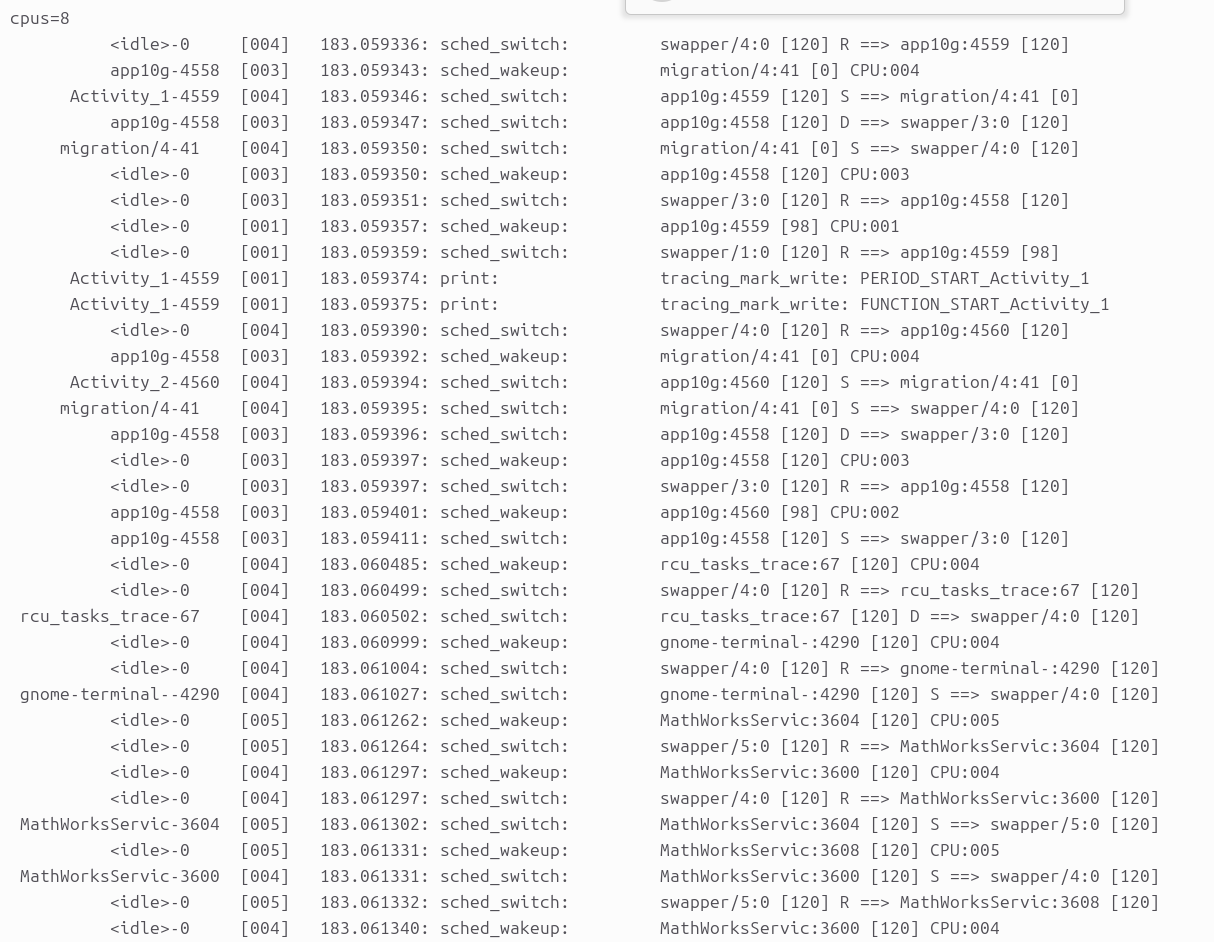
\includegraphics[width=0.80\textwidth]{Foto/Thread/trace_output.png}
	\caption{Estratto di \texttt{trace\_output.txt}: ogni riga documenta un evento di scheduling con timestamp, nome processo, PID e stato di transizione.}
	\label{fig:step2_traceoutput}
\end{figure}


% ============================================================
\subsubsection{Step 3 --- Compilazione ed Esecuzione del Parser C++}
% ============================================================

Il parser \texttt{thread\_analysis.cpp} viene compilato a runtime direttamente
nella directory di output della sessione corrente. La scelta di compilare
\emph{just-in-time} anziché distribuire un binario precompilato ha una ragione
precisa: il parser viene sviluppato reciprocamente con le applicazioni durante lo sviluppo, e
compilarlo ogni volta garantisce che venga sempre usata la versione corrispondente
al sorgente presente in \texttt{src/tools/}, senza rischio di disallineamento tra
parser e formato dei marker.

I flag \texttt{-O2 -std=c++17} bilanciano velocità di compilazione e ottimizzazione
del codice prodotto. L'eseguibile viene scritto dentro \texttt{OUTPUT\_DIR}: anche
il binario del parser fa parte degli artefatti della sessione, facilitando il
debugging in caso di risultati anomali.

\begin{lstlisting}[language=bash, caption={\texttt{run\_trace.sh} -- Step 3: compilazione e lancio del parser C++}]
	echo "[3/5] Compilazione analizzatore C++..."
	PARSER_EXE="$OUTPUT_DIR/thread_analysis"
	if [ -f "$PARSER_SRC" ]; then
	g++ -O2 -std=c++17 "$PARSER_SRC" -o "$PARSER_EXE"
	else
	echo "ATTENZIONE: File $PARSER_SRC non trovato!"
	PARSER_EXE=""
	fi
	
	echo "[4/5] Avvio Analisi (Lettura periodi dal codice)..."
	if [ -n "$PARSER_EXE" ]; then
	cd "$OUTPUT_DIR" || exit
	./thread_analysis "trace_output.txt" "$SRC_FILE_ABS" "ALL" > "risultati_finali.txt"
	echo ""
	cat "risultati_finali.txt"
\end{lstlisting}

Il parser spiegato interamente nel suo funzionamento al Capitolo \ref{threadanalysis}, riceve tre argomenti: il file di testo del trace, il sorgente
dell'applicazione (da cui estrae i periodi) e la stringa \texttt{"ALL"}
che indica di analizzare tutti i thread trovati nel log. L'output viene rediretto
in \texttt{risultati\_finali.txt} e contemporaneamente stampato a terminale
con \texttt{cat}.

\noindent\textbf{File prodotti:} \texttt{timeline.csv}, \texttt{risultati\_finali.txt}

\begin{figure}[htbp]
	\centering
	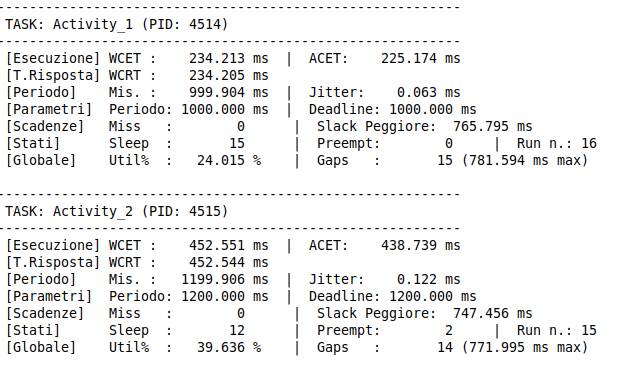
\includegraphics[width=0.60\textwidth]{Foto/Thread/risultati_finali.png}
	\caption{Output a terminale di \texttt{thread\_analysis}: metriche RT per ogni task.}
	\label{fig:step3_risultati}
\end{figure}

\paragraph*{Analisi del file \texttt{timeline.csv}}
Il file \texttt{timeline.csv} contiene tutte le misurazioni temporali dei thread e le statistiche finali estratte dal trace kernel. Nella Tabella \ref{tab:timeline_stats} è riportato il significato di ciascuna metrica statistica (identificata dal prefisso \texttt{STAT\_}) prodotta dall'analizzatore C++ e utile per valutare le prestazioni \textit{real-time} di ogni applicazione tracciata. Questo processo di analisi viene eseguito per qualsiasi script bash utilizzato durante la simulazione, come mostrato ad esempio nel listato \ref{timelineMarker.sh}. In Figura \ref{figtimeline.csv} viene riportato un esempio del risultato grafico ottenuto in seguito alla generazione del file di timeline.

\begin{figure}[htbp]
	\centering
	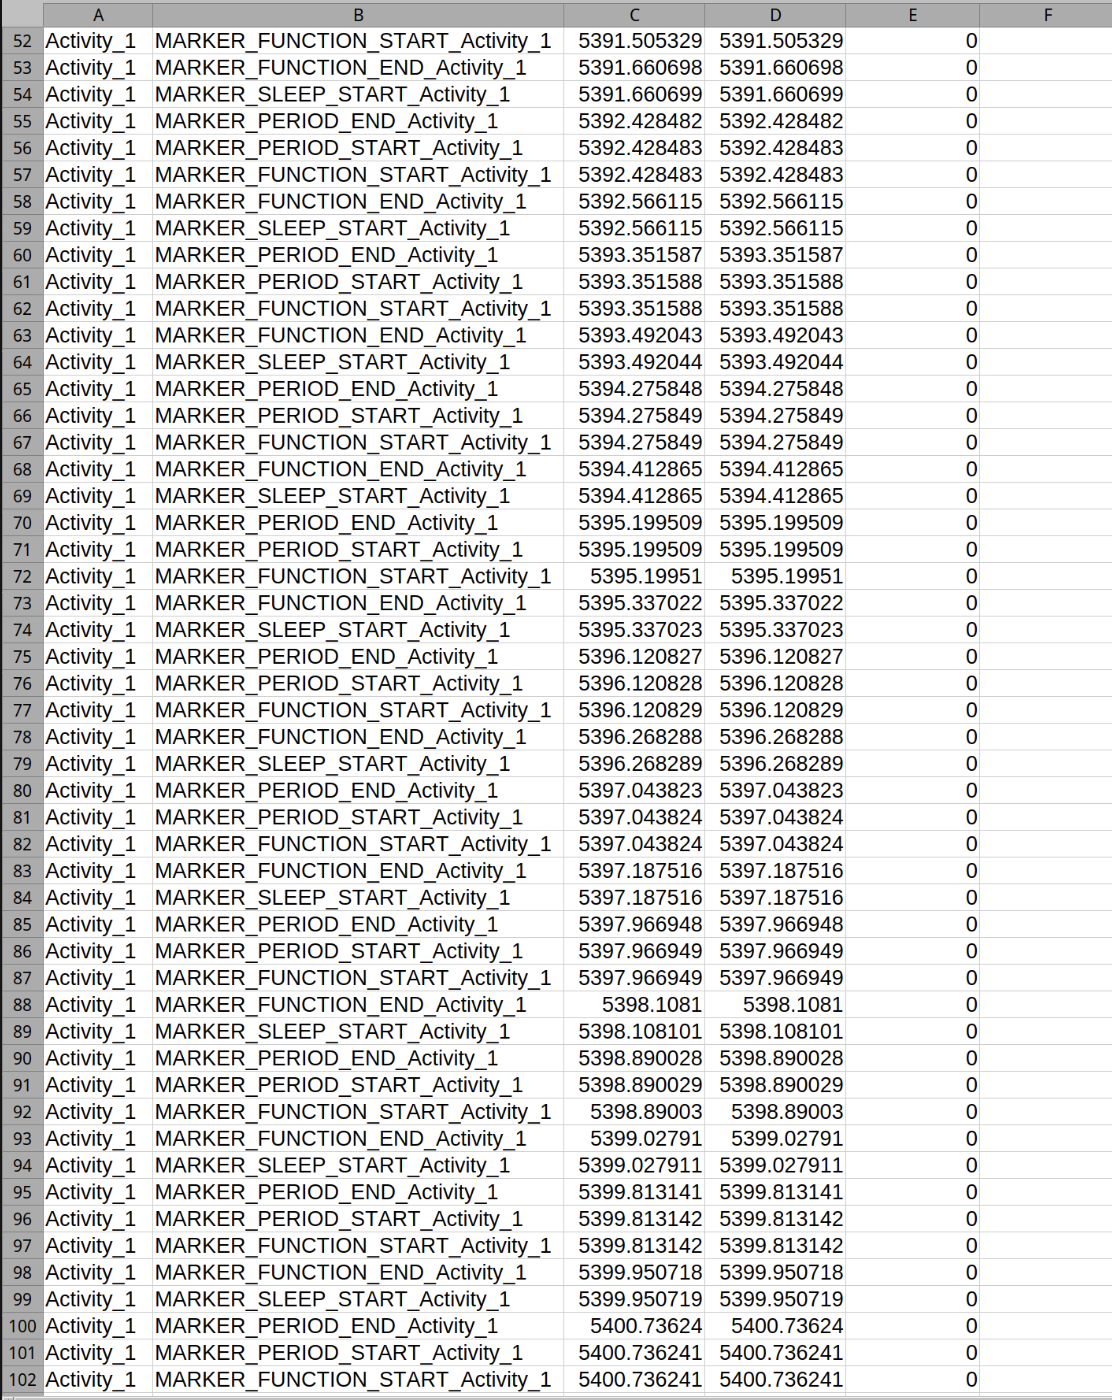
\includegraphics[width=0.55\textwidth]{Foto/Thread/Timeline.png}
	\caption{Esempio di risultato ottenuto nella creazione del file \texttt{timeline.csv}.}
	\label{figtimeline.csv}
\end{figure}

\begin{table}[H]
	\centering
	\begin{tabular}{|l|p{10cm}|}
		\hline
		\textbf{Statistica} & \textbf{Significato} \\
		\hline
		\texttt{STAT\_PERIOD} & Periodo nominale del task dichiarato a codice. \\
		\texttt{STAT\_MEASURED} & Periodo medio effettivo misurato tra due esecuzioni consecutive. \\
		\texttt{STAT\_DEADLINE} & Scadenza temporale (deadline) entro cui il task deve completare l'esecuzione. \\
		\texttt{STAT\_WCET} & \textit{Worst-Case Execution Time}: il tempo massimo di esecuzione registrato. \\
		\texttt{STAT\_ACET} & \textit{Average-Case Execution Time}: il tempo medio di esecuzione. \\
		\texttt{STAT\_JITTER} & Jitter misurato sull'attivazione o sull'esecuzione del task. \\
		\texttt{STAT\_UTIL} & Fattore di utilizzo della CPU (percentuale di tempo trascorso in esecuzione). \\
		\texttt{STAT\_NRUN} & Numero totale di attivazioni (run) del task. \\
		\texttt{STAT\_NPRE} & Numero totale di \textit{preemption} (interruzioni da parte di altri task) subite. \\
		\texttt{STAT\_NSLP} & Numero di volte in cui il task è entrato in stato di \textit{sleep}. \\
		\texttt{STAT\_NMISS} & Numero di \textit{deadline} mancate durante la sessione di tracciamento. \\
		\texttt{STAT\_WSLACK} & \textit{Worst-case slack time}: il margine temporale minimo registrato tra il termine dell'esecuzione e la deadline. \\
		\texttt{STAT\_HGAPS} & Numero di \textit{huge gaps}, ovvero anomalie in cui il task non è stato attivato per un periodo superiore alla norma. \\
		\texttt{STAT\_NGAPS} & Numero totale di gap temporali (ritardi di risveglio) rilevati. \\
		\texttt{STAT\_MAXGAP} & Durata massima registrata per un gap anomalo. \\
		\texttt{STAT\_RUNTOT} & Tempo totale in cui il task è stato attivamente in esecuzione sulla CPU. \\
		\texttt{STAT\_PRETOT} & Tempo totale trascorso in stato di \textit{preemption} (pronto per eseguire ma bloccato da task a priorità maggiore). \\
		\texttt{STAT\_SLPTOT} & Tempo totale trascorso in stato di \textit{sleep}. \\
		\hline
	\end{tabular}
	\caption{Descrizione delle metriche statistiche presenti nel file \texttt{timeline.csv}}
	\label{tab:timeline_stats}
\end{table}
% ============================================================
\subsubsection{Step 4 --- Monitor Visivo Python e Chiusura}
% ============================================================

L'ultimo passo della pipeline lancia \texttt{monitor.py} passandogli il file
\texttt{timeline.csv} generato dal parser. Lo script Python legge le colonne
del CSV (timestamp di inizio e fine di ogni finestra temporale per ogni thread)
e produce un diagramma di Gantt che rende immediatamente visibili i periodi, le
durate di esecuzione, i tempi di sleep e le eventuali anomalie temporali.

\begin{lstlisting}[language=bash, caption={\texttt{run\_trace.sh} -- Step 4: monitor visivo e banner finale}]
	echo "[5/5] Avvio monitor visivo (Python)..."
	if [ -f "$MONITOR_SCRIPT_ABS" ]; then
	python3 "$MONITOR_SCRIPT_ABS" "timeline.csv"
	else
	echo "ATTENZIONE: Non trovo lo script $MONITOR_SCRIPT_ABS."
	fi
	cd "$PROJECT_ROOT" || exit
	fi
	
	echo "========================================================="
	echo "Tracciamento completato! Dati in: $OUTPUT_DIR"
\end{lstlisting}

\noindent\textbf{File prodotto:} \texttt{timeline\_monitor.png}

\begin{figure}[htbp]
	\centering
	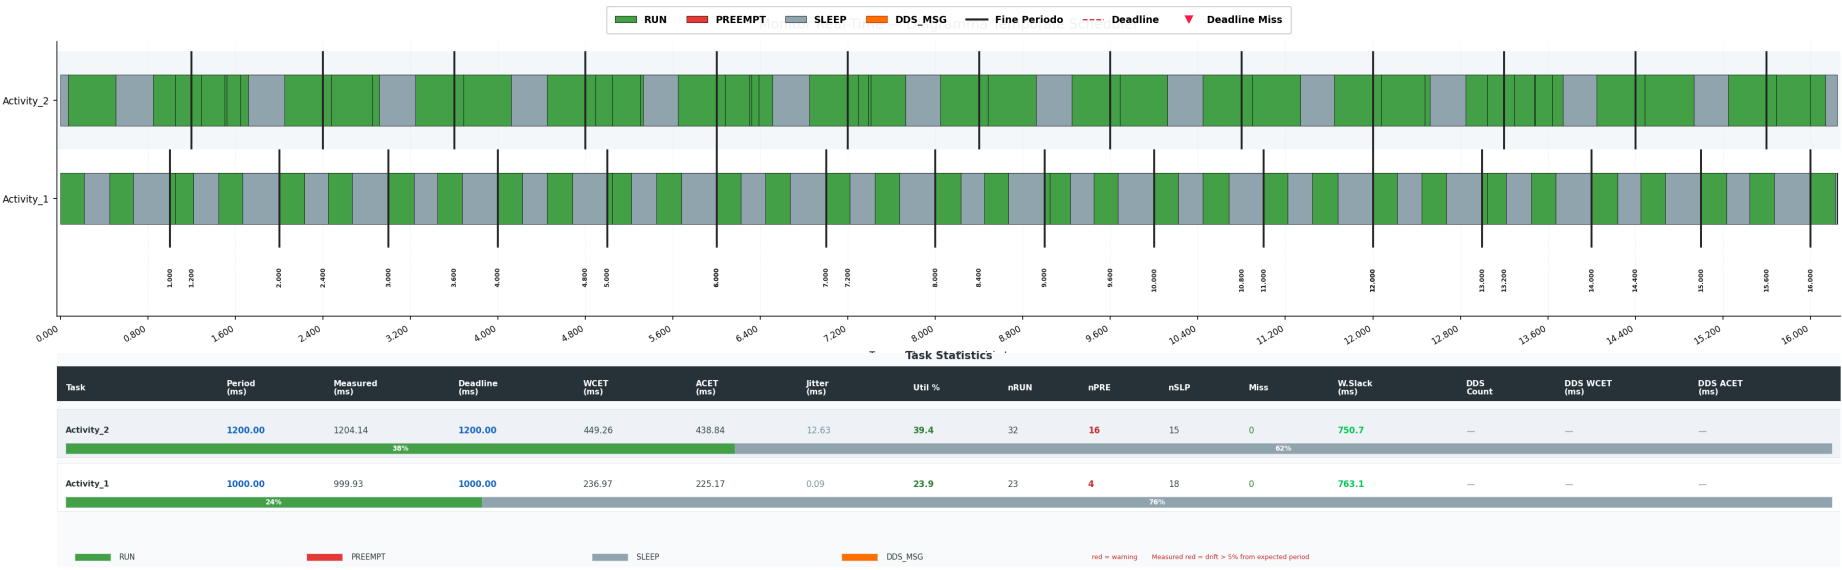
\includegraphics[width=\textwidth]{Foto/Thread/monitorapp10g.png}
	\caption{Diagramma di Gantt generato da \texttt{monitor.py} per \texttt{app10g}.}
	\label{fig:step4_monitor}
\end{figure}



% ============================================================
\subsection{Tracciamento Passivo Multi-Processo: \texttt{marker.sh}}
\label{timelineMarker.sh}
% ============================================================

\noindent\textbf{Posizione nel progetto:} \texttt{bin/tools/marker.sh}

\bigskip

A differenza di \texttt{run\_trace.sh}, che lancia l'eseguibile e lo registra
in un unico processo, \texttt{marker.sh} opera in modalità \textbf{passiva}: i
processi da osservare sono già in esecuzione in terminali separati prima che lo
script venga invocato. Il suo compito è agganciare il tracer kernel a quei
processi esistenti senza interromperne l'esecuzione. Viene invocato con i nomi
degli eseguibili già avviati:

\begin{lstlisting}[language=bash]
	./marker.sh Broadcastner Listener
\end{lstlisting}

Questo approccio è necessario per le applicazioni distribuite: \texttt{Broadcastner}
e \texttt{Listener} devono partire contemporaneamente (su terminali distinti o
nodi distinti) e completare la fase di discovery DDS tra di loro prima che
l'osservazione abbia senso. Solo una volta che i due nodi si sono scoperti e il
flusso di messaggi è attivo, si aggancia il tracer.

% ============================================================
\subsubsection{Risoluzione dei Percorsi e Lettura degli Argomenti}
% ============================================================

Le prime righe sono identiche a \texttt{run\_trace.sh}: calcolo di
\texttt{PROJECT\_ROOT} tramite \texttt{BASH\_SOURCE[0]} e normalizzazione dei
nomi storici tramite \texttt{resolve\_app\_name}. La differenza principale è
nella lettura degli argomenti: lo script accetta fino a due nomi di eseguibili,
permettendo il tracciamento congiunto di due processi distinti nella stessa
sessione.

\begin{lstlisting}[language=bash, caption={\texttt{marker.sh} -- Percorsi, alias e lettura argomenti}]
#!/bin/bash
# marker.sh - Estrazione TID e tracciamento passivo (standard app version)

# Salviamo la cartella principale del progetto
SCRIPT_DIR="$(cd "$(dirname "${BASH_SOURCE[0]}")" && pwd)"
PROJECT_ROOT="$(cd "$SCRIPT_DIR/../.." && pwd)"

# Se siamo già root (es. dashboard), non serve sudo
if [ "$EUID" -eq 0 ]; then
SUDO_CMD=""
else
SUDO_CMD="sudo"
fi
BASE_DIR="$PROJECT_ROOT"

# Funzione per risolvere alias dei nomi
resolve_app_name() {
	case $1 in
	GeometryBroadcastner) echo "Broadcastner" ;;
	GeometryListener)    echo "Listener" ;;
	*)                    echo "$1" ;;
	esac
}

# Chiediamo gli eseguibili (devono essere GIÀ AVVIATI negli altri terminali)
if [ "$#" -eq 0 ]; then
read -p "Inserisci il PRIMO eseguibile (già avviato, es. Broadcastner o app10f): " RAW_NAME
read -p "[Opzionale] Inserisci il SECONDO eseguibile: " RAW_SEC_NAME
else
RAW_NAME=$1
RAW_SEC_NAME=$2
fi

EXECUTABLE_NAME=$(resolve_app_name "$RAW_NAME")
APP_NAME=$(basename "$EXECUTABLE_NAME")


\end{lstlisting}

% ============================================================
\subsubsection{Aggancio Passivo: Estrazione dei TID da \texttt{/proc}}
% ============================================================

Il cuore dello script è la funzione \texttt{aggiungi\_pid\_e\_thread}, che
implementa la logica di aggancio passivo. Il problema da risolvere è il
seguente: \texttt{trace-cmd record} accetta il flag \texttt{-P} per filtrare gli
eventi di un processo specifico, ma se si specifica solo il PID del processo
padre si perdono gli eventi dei thread interni, che hanno TID distinti dal PID
padre. La soluzione è navigare il filesystem virtuale \texttt{/proc/[PID]/task/}: il
kernel Linux espone lì una directory per ogni thread del processo, il cui nome è
il TID. Per ognuno, il file \texttt{comm} contiene il nome leggibile del thread
(quello assegnato con \texttt{pthread\_setname\_np}). La funzione costruisce
incrementalmente la stringa \texttt{PIDS\_CMD} aggiungendo un flag \texttt{-P}
per ogni TID trovato.

\begin{lstlisting}[language=bash, caption={\texttt{marker.sh} -- Estrazione ricorsiva dei TID da /proc}]

# ESTRAZIONE DEI THREAD (TID)

PIDS_1=$(pidof "$APP_NAME")
if [ -z "$PIDS_1" ]; then
echo "ERRORE: Il processo '$APP_NAME' non è in esecuzione!"
echo "Avvia prima l'app in un altro terminale, poi lancia questo script."
echo ""
echo "  Per le app DDS (Broadcastner, Listener, ecc.) serve sudo:"
echo "    sudo ./$APP_NAME"
exit 1
fi

PIDS_CMD=""

# Funzione per estrarre tutti i thread
aggiungi_pid_e_thread() {
	local process_name=$1
	local pids=$2
	for p in $pids; do
	PIDS_CMD="$PIDS_CMD -P $p"
	echo ">> Trovato processo principale: $process_name (PID: $p)"
	
	# Esploriamo /proc/$p/task/ per trovare tutti i thread interni (TID)
	if [ -d "/proc/$p/task" ]; then
	for tid_path in /proc/$p/task/*; do
	tid=$(basename "$tid_path")
	if [ "$tid" != "$p" ]; then
	PIDS_CMD="$PIDS_CMD -P $tid"
	# Leggiamo il nome del thread per conferma a video
	thread_name=$(cat "$tid_path/comm" 2>/dev/null)
	echo "   -> Agganciato thread: $thread_name (TID: $tid)"
	fi
	done
	fi
	done
}
\end{lstlisting}

La funzione viene chiamata prima per il processo primario, poi, se è stato
fornito un secondo argomento, anche per il processo secondario. In entrambi i
casi, se il processo non è trovato in esecuzione, lo script lo segnala con un
avviso ma non termina: il tracciamento del primo processo continua comunque.

\begin{lstlisting}[language=bash, caption={\texttt{marker.sh} -- Chiamata per primo e secondo processo}]
	# 1. Processiamo la prima app e i suoi thread
	aggiungi_pid_e_thread "$APP_NAME" "$PIDS_1"
	
	# 2. Se e' presente un secondo eseguibile, lo si cerca insieme ai suoi thread
	if [ -n "$RAW_SEC_NAME" ]; then
	SEC_EXECUTABLE_NAME=$(resolve_app_name "$RAW_SEC_NAME")
	SEC_APP_NAME=$(basename "$SEC_EXECUTABLE_NAME")
	PIDS_2=$(pidof "$SEC_APP_NAME")
	if [ -n "$PIDS_2" ]; then
	echo "---------------------------------------------------------"
	aggiungi_pid_e_thread "$SEC_APP_NAME" "$PIDS_2"
	echo ">> Tracciamento congiunto pronto."
	else
	echo ">> ATTENZIONE: '$SEC_APP_NAME' non trovato. Traccio solo $APP_NAME."
	fi
	else
	echo ">> Tracciamento singolo pronto."
	fi
\end{lstlisting}

\begin{figure}[htbp]
	\centering
	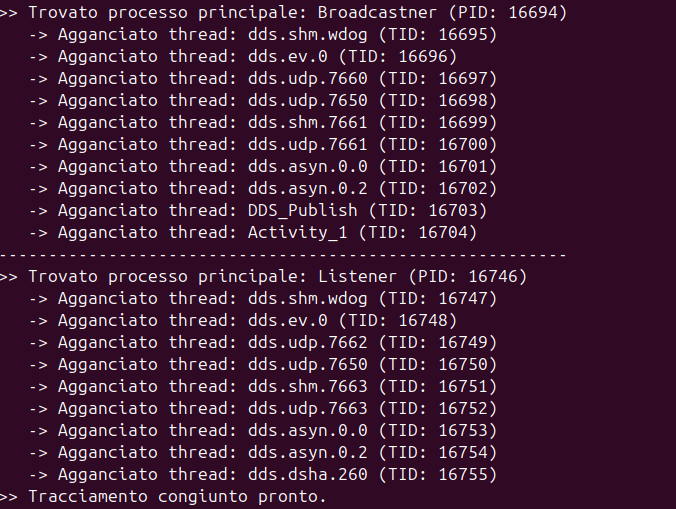
\includegraphics[width=0.80\textwidth]{Foto/Thread/TidBroadcastner.png}
	\caption{Output di \texttt{marker.sh}: aggancio congiunto con estrazione di tutti i TID prima di avviare il trace.}
	\label{fig:marker_aggancio}
\end{figure}

% ============================================================
\subsubsection{Discovery del Sorgente, Directory di Output e Registrazione}
% ============================================================

Completata la costruzione di \texttt{PIDS\_CMD}, lo script cerca il sorgente
C/C++ dell'applicazione con la stessa funzione \texttt{find\_src} vista in
\texttt{run\_trace.sh}, crea la directory di sessione con timestamp e poi avvia
\texttt{trace-cmd record}. La differenza cruciale rispetto a \texttt{run\_trace.sh}
è che in tale sede non viene passato alcun eseguibile alla fine del comando: la
registrazione non lancia nulla, ma filtra gli eventi del kernel esclusivamente
sui PID e TID elencati in \texttt{PIDS\_CMD}. La registrazione rimane attiva
finché l'utente preme \texttt{Ctrl+C}.

\begin{lstlisting}[language=bash, caption={\texttt{marker.sh} -- Discovery sorgente, output e registrazione passiva}]
# Troviamo il file sorgente per l'analisi
find_src() {
	local name=$1
	# Priorità a src/app/
	local candidate=$(find "$PROJECT_ROOT/src/app" -name "${name}.cpp" -o -name "${name}.c" | head -n 1)
	if [ -n "$candidate" ]; then
	echo "$candidate"
	else
	# Cerca ovunque in src/
	find "$PROJECT_ROOT/src" -name "${name}.cpp" -o -name "${name}.c" | head -n 1
	fi
}

SRC_FILE=$(find_src "$APP_NAME")

if [ ! -f "$SRC_FILE" ]; then
echo "ERRORE CRITICO: Non trovo il file sorgente per $APP_NAME!"
exit 1
fi

SRC_FILE_ABS="$SRC_FILE"
MONITOR_SCRIPT_ABS="$PROJECT_ROOT/src/tools/monitor.py"
PARSER_SRC="$PROJECT_ROOT/src/tools/thread_analysis.cpp"

TIMESTAMP=$(date +"%Y%m%d_%H%M%S")
OUTPUT_DIR="$PROJECT_ROOT/bin/Test/trace_marker_${APP_NAME}_${TIMESTAMP}"

echo "========================================================="
echo " Inizio tracciamento per: $APP_NAME"
echo " Sorgente trovato: $SRC_FILE_ABS"
echo " Cartella di output: $OUTPUT_DIR"
echo "========================================================="

mkdir -p "$OUTPUT_DIR"

echo "[1/5] Registrazione trace-cmd sui PID e THREAD scelti..."
echo "--- PREMI Ctrl+C PER FERMARE LA REGISTRAZIONE QUANDO HAI FINITO! ---"
# Lanciamo trace-cmd in background e catturiamo il suo PID per gestire il segnale
TRACE_CMD_PID=""
cleanup() {
	echo ""
	echo "--- Segnale ricevuto, arresto trace-cmd... ---"
	if [ -n "$TRACE_CMD_PID" ] && kill -0 "$TRACE_CMD_PID" 2>/dev/null; then
	kill -INT "$TRACE_CMD_PID" 2>/dev/null
	wait "$TRACE_CMD_PID" 2>/dev/null
	fi
}
trap cleanup INT TERM

$SUDO_CMD trace-cmd record -e sched:sched_switch -e sched:sched_wakeup $PIDS_CMD -o "$OUTPUT_DIR/trace.dat" &
TRACE_CMD_PID=$!
wait $TRACE_CMD_PID 2>/dev/null
trap - INT TERM

if [ ! -f "$OUTPUT_DIR/trace.dat" ]; then
echo "ERRORE CRITICO: trace.dat non creato."
exit 1
fi

$SUDO_CMD chown -R "${SUDO_UID:-$(id -u)}:${SUDO_GID:-$(id -g)}" "$OUTPUT_DIR"
\end{lstlisting}

% ============================================================
\subsubsection{Decodifica, Analisi, Monitor e KernelShark}
% ============================================================

I passi 2, 3, 4 e 5 sono identici a \texttt{run\_trace.sh}: decodifica del
binario in testo, compilazione just-in-time del parser C++ e suo lancio,
visualizzazione con il monitor Python. \texttt{marker.sh} aggiunge però un sesto
passo che \texttt{run\_trace.sh} non ha: l'apertura automatica di KernelShark.

\begin{lstlisting}[language=bash, caption={\texttt{marker.sh} -- Decodifica, analisi, monitor e apertura KernelShark}]
	echo "[2/5] Generazione del report testuale..."
	trace-cmd report "$OUTPUT_DIR/trace.dat" > "$OUTPUT_DIR/trace_output.txt"
	
	echo "[3/5] Compilazione analizzatore C++..."
	PARSER_EXE="$OUTPUT_DIR/thread_analysis"
	if [ -f "$PARSER_SRC" ]; then
	g++ -O2 -std=c++17 "$PARSER_SRC" -o "$PARSER_EXE"
	else
	echo "ATTENZIONE: File $PARSER_SRC non trovato!"
	PARSER_EXE=""
	fi
	
	echo "[4/5] Avvio Analisi (Lettura periodi dal codice)... "
	if [ -n "$PARSER_EXE" ]; then
	cd "$OUTPUT_DIR" || exit
	./thread_analysis "trace_output.txt" "$SRC_FILE_ABS" "ALL" > "risultati_finali.txt"
	echo ""
	cat "risultati_finali.txt"
	
	echo "[5/5] Avvio monitor visivo (Python)..."
	if [ -f "$MONITOR_SCRIPT_ABS" ]; then
	PYTHON_BIN="python3"
	"$PYTHON_BIN" "$MONITOR_SCRIPT_ABS" "timeline.csv"
	else
	echo "ATTENZIONE: Non trovo lo script $MONITOR_SCRIPT_ABS."
	fi
	cd "$PROJECT_ROOT" || exit
	fi
	
	echo "========================================================="
	echo "Tracciamento completato! Dati in: $OUTPUT_DIR"
	
	echo "[6/6] Avvio KernelShark..."
	if command -v kernelshark >/dev/null 2>&1; then
	(cd "$OUTPUT_DIR" && kernelshark trace.dat) &
	else
	echo "ATTENZIONE: KernelShark non trovato."
	fi
\end{lstlisting}

KernelShark viene lanciato in background (\texttt{\&}) all'interno di una
subshell che prima cambia directory nella cartella di output. In questo modo
KernelShark trova \texttt{trace.dat} nella propria directory di lavoro e può
aprirlo direttamente senza percorso assoluto. L'operatore \texttt{\&} lascia
libero il terminale: lo script termina e stampa il banner finale, mentre
KernelShark rimane aperto come processo separato.

\begin{figure}[H]
	\centering
	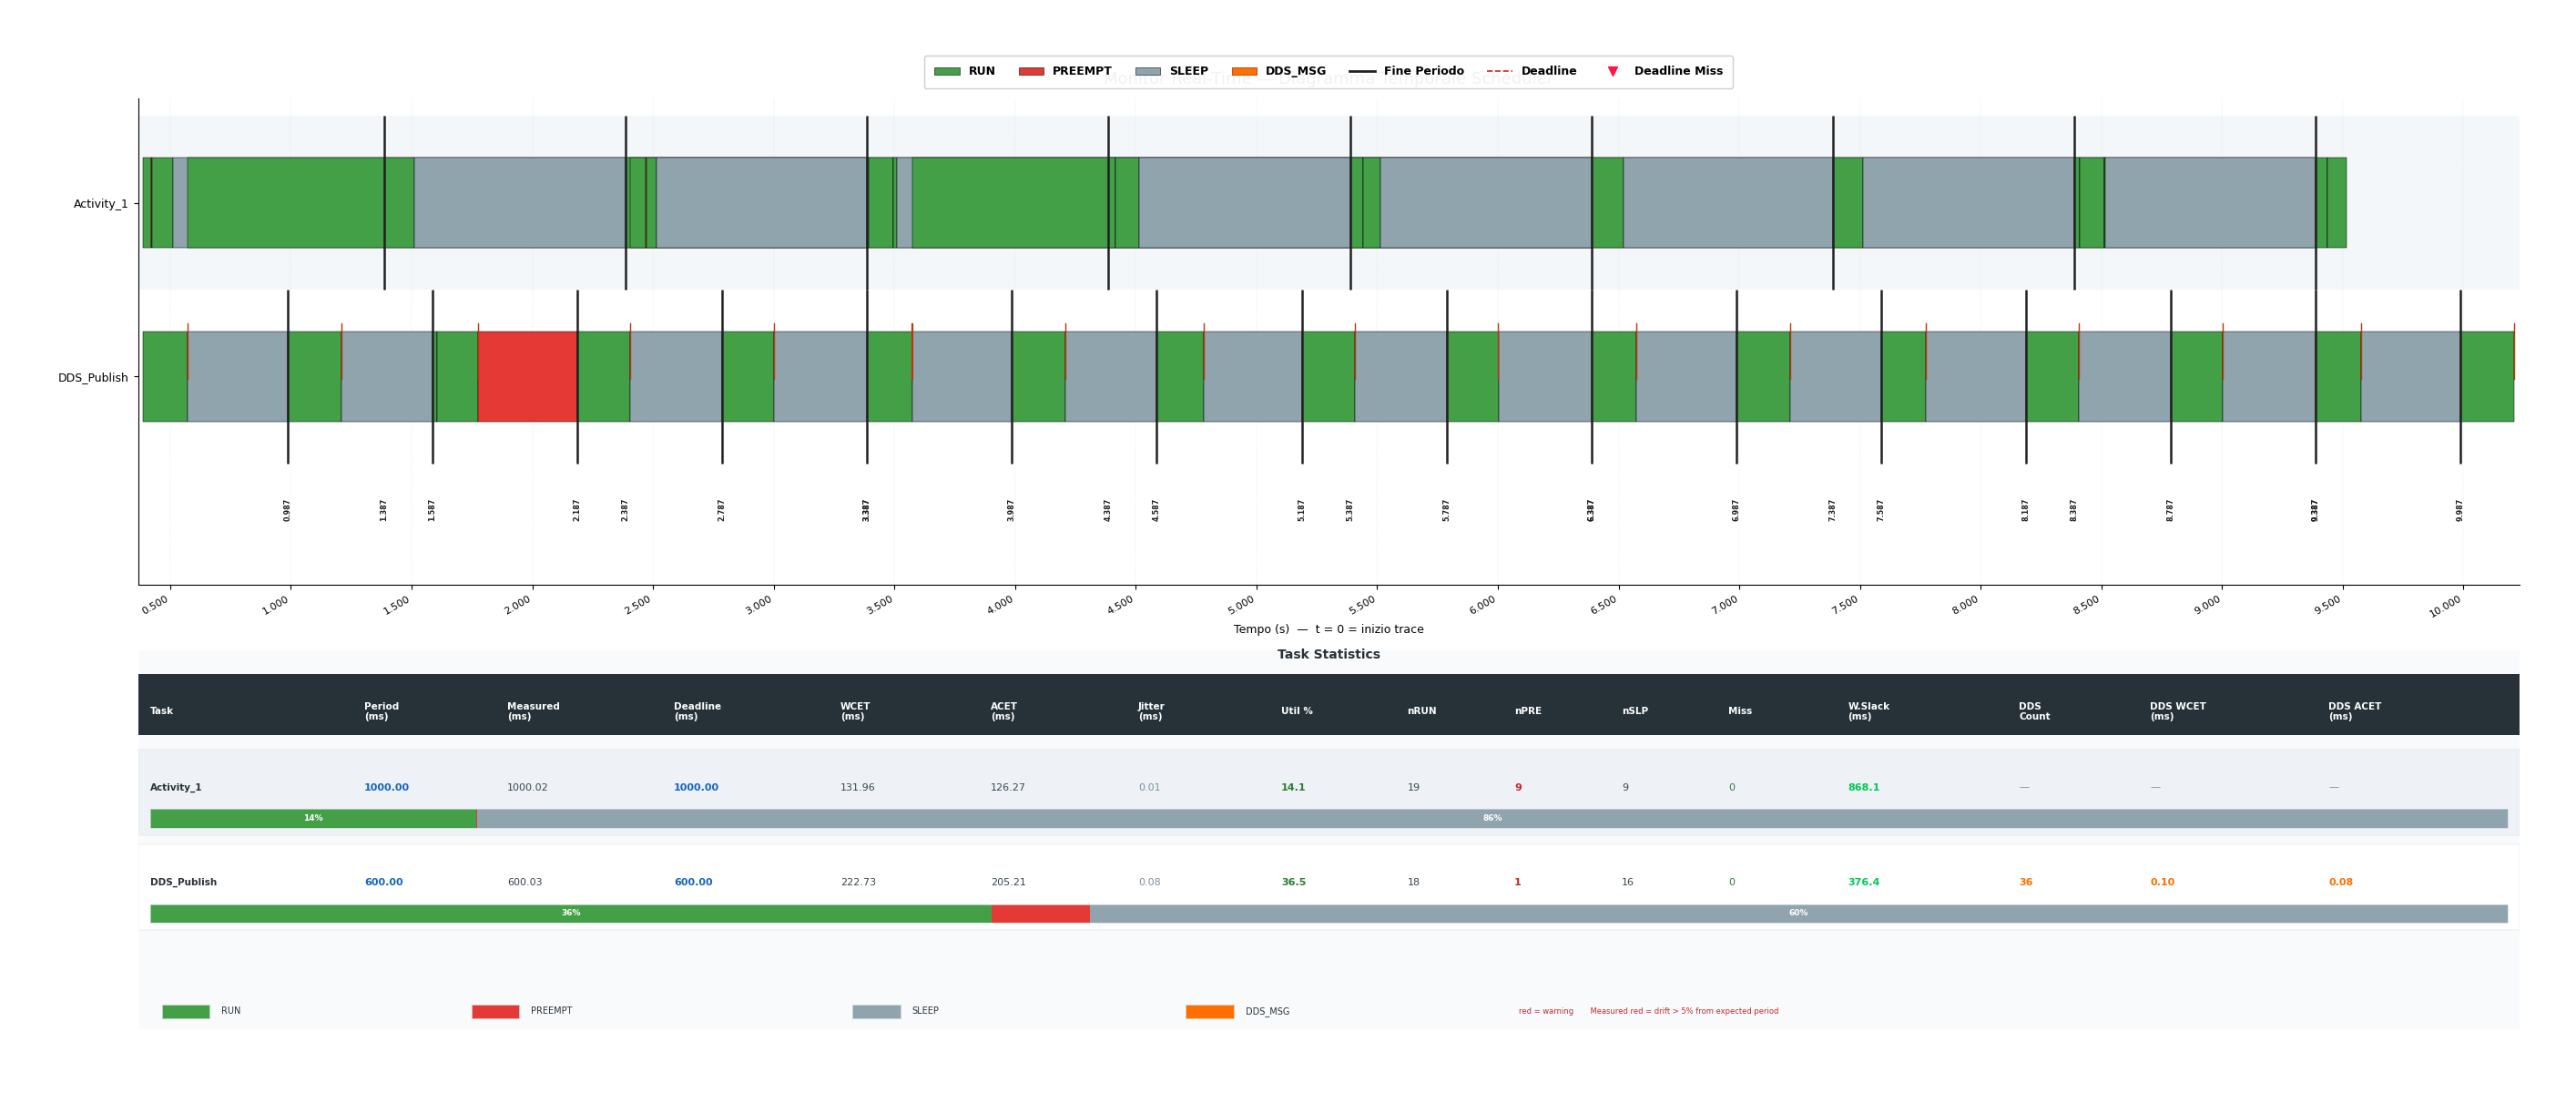
\includegraphics[width=\textwidth]{Foto/Thread/MonitorBroadcastner.png}
	\caption{Monitor Python con risultato della simulazione Broadcastner--Listener. Si può notare nel monitor la barra arancio riguardante il tempo impiegato per la comunicazione DDS.}
	\label{fig:monitoreprosima}
\end{figure}


\begin{figure}[H]
	\centering
	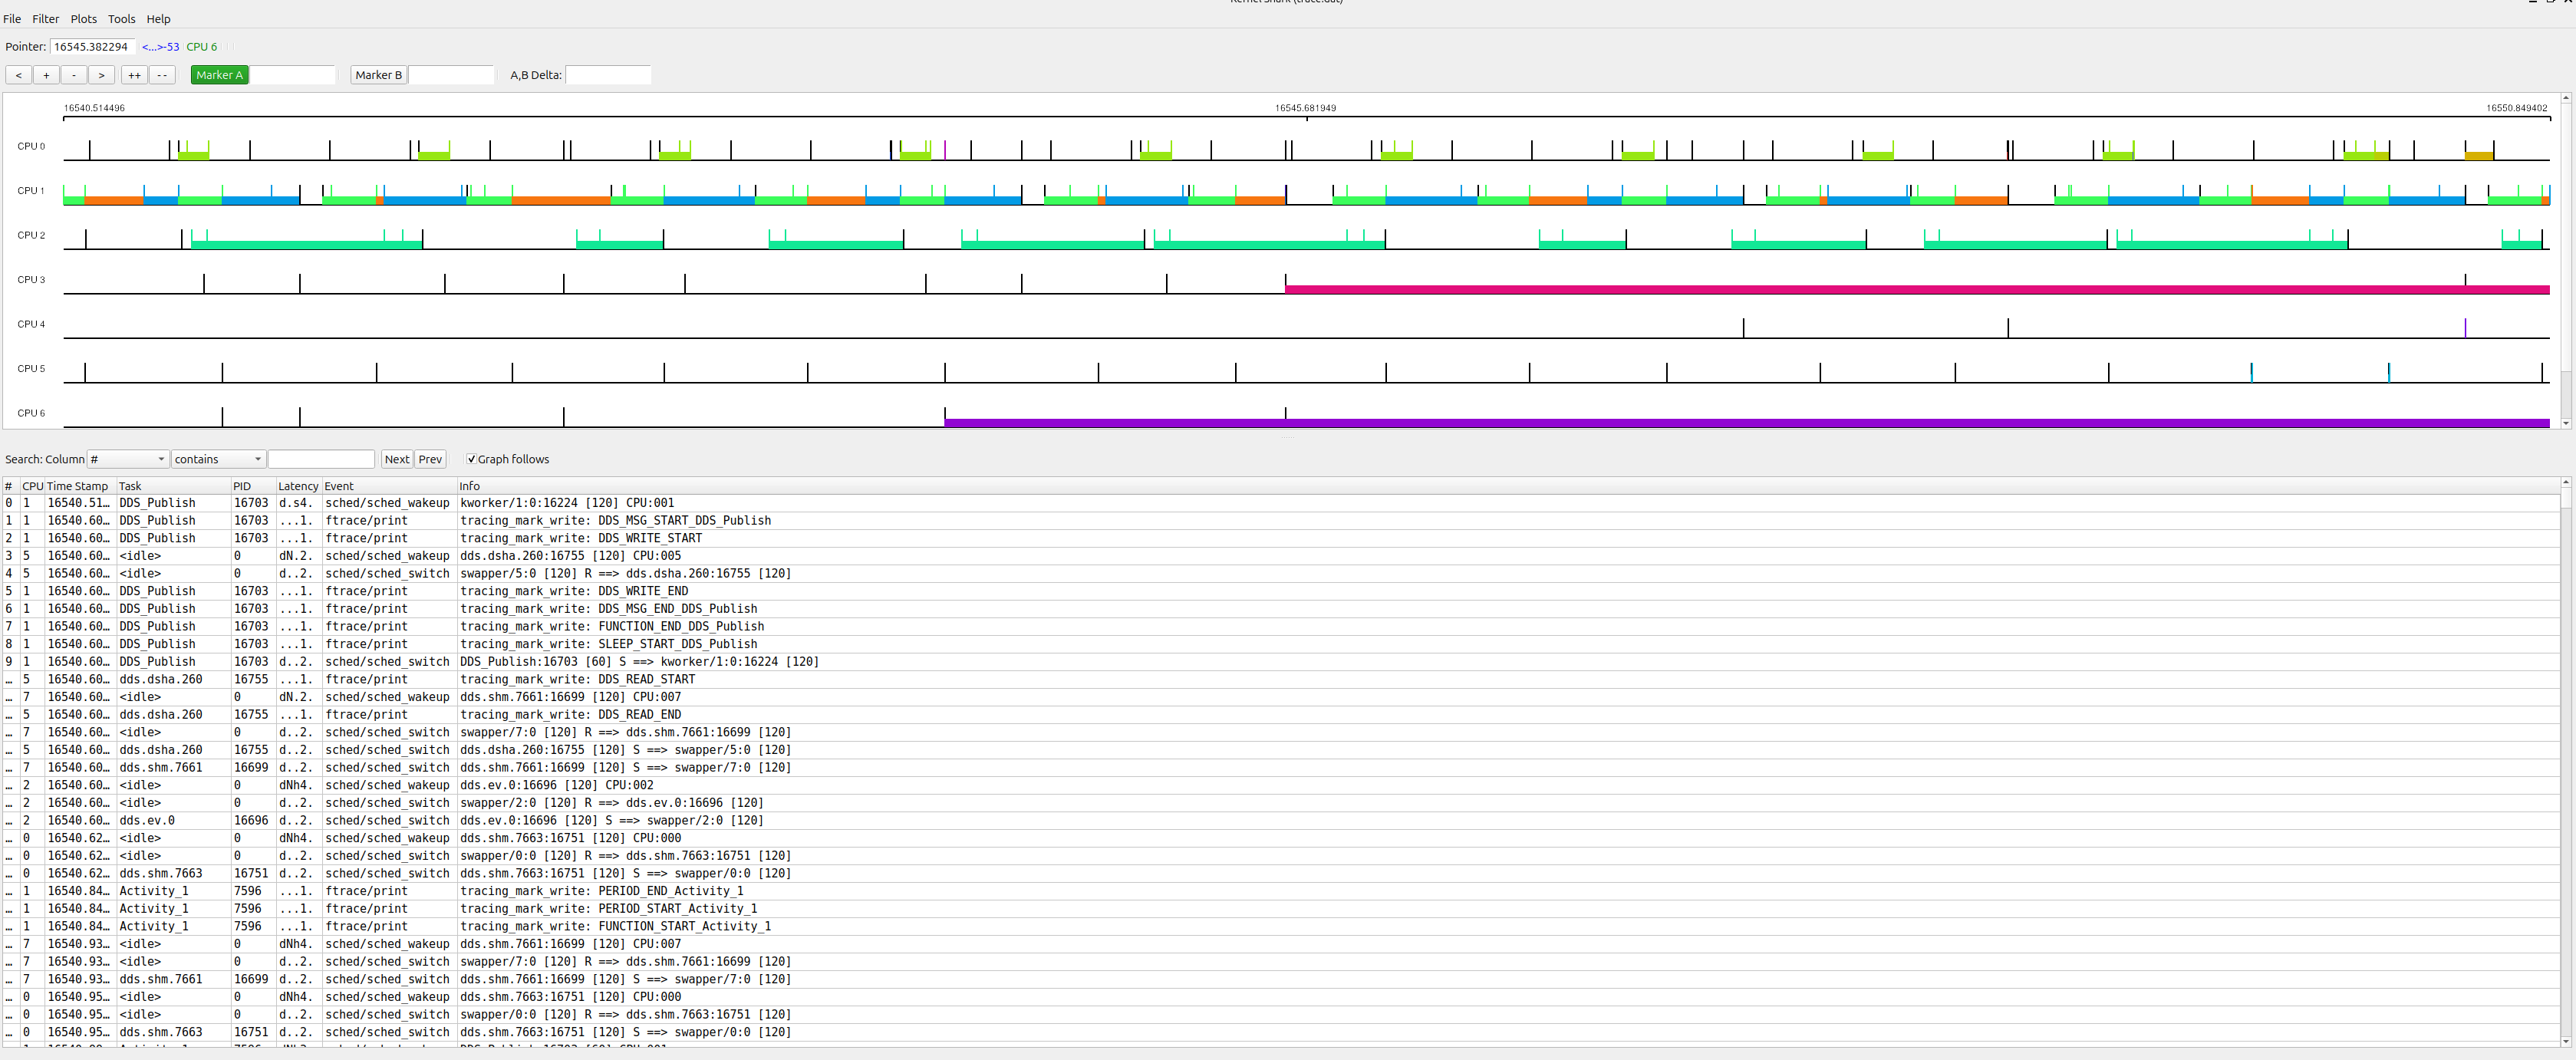
\includegraphics[width=\textwidth]{Foto/Thread/SharkBroadcastner}
	\caption{Interfaccia KernelShark con marker applicativi visibili sulla timeline.}
	\label{fig:kernelshark_fase4}
\end{figure}

\clearpage

% ============================================================
\subsection{Le Versioni Didattiche: \texttt{marker1.sh} -- \texttt{marker4.sh}}
% ============================================================

\noindent\textbf{Posizione nel progetto:} \texttt{bin/tools/marker1.sh},
\texttt{marker2.sh}, \texttt{marker3.sh}, \texttt{marker4.sh}

\bigskip

La logica di \texttt{marker.sh} è suddivisa in quattro script indipendenti che
eseguono esattamente gli stessi passi nell'identico ordine, ma separati in
processi distinti. Il valore aggiunto non è funzionale ma didattico e diagnostico:
ogni step può essere eseguito individualmente, ispezionato, ripetuto o saltato.
Se ad esempio il parser produce risultati anomali, si può rieseguire solo
\texttt{marker3.sh} su una cartella di sessione già esistente senza dover
ripetere la registrazione. Il meccanismo che tiene insieme i quattro script
è il file temporaneo \texttt{/tmp/last\_marker\_dir}.

% ------------------------------------------------------------
\subsubsection{\texttt{marker1.sh}: Registrazione}
% ------------------------------------------------------------

\texttt{marker1.sh} contiene la logica completa di aggancio TID, creazione della
directory di output e avvio di \texttt{trace-cmd record}. Al termine, invece di
procedere con i passi successivi, scrive il percorso della cartella di output in
\texttt{/tmp/last\_marker\_dir} e il nome dell'applicazione in
\texttt{app\_name.txt} dentro la stessa cartella. Questi due file fungono da
canale di comunicazione verso gli script successivi: ogni script successivo legge
da lì il contesto della sessione corrente.

\begin{lstlisting}[language=bash, caption={\texttt{marker1.sh} -- Aggancio TID, registrazione e salvataggio contesto}]
	#!/bin/bash
	# marker1.sh - Estrazione TID e tracciamento passivo (Registrazione)
	
	SCRIPT_DIR="$(cd "$(dirname "${BASH_SOURCE[0]}")" && pwd)"
	PROJECT_ROOT="$(cd "$SCRIPT_DIR/../.." && pwd)"
	
	# Funzione per risolvere alias dei nomi
	resolve_app_name() {
		case $1 in
		GeometryBroadcastner) echo "Broadcastner" ;;
		GeometryListener)    echo "Listener" ;;
		*)                    echo "$1" ;;
		esac
	}
	
	if [ "$#" -eq 0 ]; then
	read -p "Inserisci il PRIMO eseguibile (già avviato, es. Broadcastner o app10f): " RAW_NAME
	read -p "[Opzionale] Inserisci il SECONDO eseguibile: " RAW_SEC_NAME
	else
	RAW_NAME=$1
	RAW_SEC_NAME=$2
	fi
	
	EXECUTABLE_NAME=$(resolve_app_name "$RAW_NAME")
	APP_NAME=$(basename "$EXECUTABLE_NAME")
	
	PIDS_1=$(pidof "$APP_NAME")
	if [ -z "$PIDS_1" ]; then
	echo "ERRORE: Il processo '$APP_NAME' non è in esecuzione!"
	exit 1
	fi
	
	PIDS_CMD=""
	
	aggiungi_pid_e_thread() {
		local process_name=$1
		local pids=$2
		for p in $pids; do
		PIDS_CMD="$PIDS_CMD -P $p"
		echo ">> Trovato processo principale: $process_name (PID: $p)"
		if [ -d "/proc/$p/task" ]; then
		for tid_path in /proc/$p/task/*; do
		tid=$(basename "$tid_path")
		if [ "$tid" != "$p" ]; then
		PIDS_CMD="$PIDS_CMD -P $tid"
		thread_name=$(cat "$tid_path/comm" 2>/dev/null)
		echo "   -> Agganciato thread: $thread_name (TID: $tid)"
		fi
		done
		fi
		done
	}
	
	aggiungi_pid_e_thread "$APP_NAME" "$PIDS_1"
	
	if [ -n "$RAW_SEC_NAME" ]; then
	SEC_EXECUTABLE_NAME=$(resolve_app_name "$RAW_SEC_NAME")
	SEC_APP_NAME=$(basename "$SEC_EXECUTABLE_NAME")
	PIDS_2=$(pidof "$SEC_APP_NAME")
	if [ -n "$PIDS_2" ]; then
	aggiungi_pid_e_thread "$SEC_APP_NAME" "$PIDS_2"
	fi
	fi
	
	TIMESTAMP=$(date +"%Y%m%d_%H%M%S")
	OUTPUT_DIR="$PROJECT_ROOT/bin/Test/trace_marker_${APP_NAME}_${TIMESTAMP}"
	mkdir -p "$OUTPUT_DIR"
	
	# Salviamo la cartella di output per i prossimi script
	echo "$OUTPUT_DIR" > /tmp/last_marker_dir
	# Salviamo anche l'app name per trovare il sorgente in marker3
	echo "$APP_NAME" > "$OUTPUT_DIR/app_name.txt"
	
	echo "========================================================="
	echo " Inizio tracciamento per: $APP_NAME"
	echo " Cartella di output: $OUTPUT_DIR"
	echo "========================================================="
	
	echo "[1/4] Registrazione trace-cmd..."
	echo "--- PREMI Ctrl+C PER FERMARE LA REGISTRAZIONE ---"
	sudo trace-cmd record -e sched:sched_switch -e sched:sched_wakeup $PIDS_CMD -o "$OUTPUT_DIR/trace.dat"
	
	if [ ! -f "$OUTPUT_DIR/trace.dat" ]; then
	echo "ERRORE: trace.dat non creato."
	exit 1
	fi
	
	sudo chown -R "${SUDO_UID:-$(id -u)}:${SUDO_GID:-$(id -g)}" "$OUTPUT_DIR"
	echo "Registrazione completata. Usa marker2.sh per generare il report."
\end{lstlisting}

\noindent\textbf{File prodotti:} \texttt{trace.dat},
\texttt{/tmp/last\_marker\_dir}, \texttt{app\_name.txt}

% ------------------------------------------------------------
\subsubsection{\texttt{marker2.sh}: Decodifica}
% ------------------------------------------------------------

\texttt{marker2.sh} legge il percorso della cartella di sessione da
\texttt{/tmp/last\_marker\_dir}, ma accetta anche un argomento esplicito:
\texttt{\$\{1:-\$DEFAULT\_DIR\}} usa il primo argomento se presente, altrimenti
cade sul valore letto dal file temporaneo. Questo permette di puntare
manualmente a una sessione precedente senza dover rieseguire la registrazione.
Decodifica il binario \texttt{trace.dat} in testo e guida l'utente al passo
successivo.

\begin{lstlisting}[language=bash, caption={\texttt{marker2.sh} -- Decodifica con fallback esplicito}]
#!/bin/bash
# marker2.sh - Generazione report testuale

if [ -f /tmp/last_marker_dir ]; then
DEFAULT_DIR=$(cat /tmp/last_marker_dir)
fi

OUTPUT_DIR=${1:-$DEFAULT_DIR}

if [ -z "$OUTPUT_DIR" ] || [ ! -d "$OUTPUT_DIR" ]; then
echo "ERRORE: Cartella di output non trovata. Esegui prima marker1.sh o specifica la cartella come argomento."
exit 1
fi

echo "[2/4] Generazione del report testuale in $OUTPUT_DIR..."
if [ ! -f "$OUTPUT_DIR/trace.dat" ]; then
echo "ERRORE: $OUTPUT_DIR/trace.dat non trovato."
exit 1
fi

trace-cmd report "$OUTPUT_DIR/trace.dat" > "$OUTPUT_DIR/trace_output.txt"
echo "Report generato: $OUTPUT_DIR/trace_output.txt"
echo "Usa marker3.sh per l'analisi dei thread."
\end{lstlisting}

\noindent\textbf{File prodotto:} \texttt{trace\_output.txt}

% ------------------------------------------------------------
\subsubsection{\texttt{marker3.sh}: Analisi con Parser C++}
% ------------------------------------------------------------

\texttt{marker3.sh} recupera il nome dell'applicazione da \texttt{app\_name.txt}
(scritto da \texttt{marker1.sh}) per ricostruire il percorso del sorgente C/C++
tramite \texttt{find\_src}. Compila il parser just-in-time nella cartella di
sessione e lo esegue. La dipendenza da \texttt{trace\_output.txt} è verificata
esplicitamente: se il file non esiste, lo script segnala all'utente di eseguire
prima \texttt{marker2.sh}.

\begin{lstlisting}[language=bash, caption={\texttt{marker3.sh} -- Compilazione parser e analisi con verifica dipendenze}]
	#!/bin/bash
	# marker3.sh - Analisi dei thread con thread_analysis
	
	SCRIPT_DIR="$(cd "$(dirname "${BASH_SOURCE[0]}")" && pwd)"
	PROJECT_ROOT="$(cd "$SCRIPT_DIR/../.." && pwd)"
	
	if [ -f /tmp/last_marker_dir ]; then
	DEFAULT_DIR=$(cat /tmp/last_marker_dir)
	fi
	
	OUTPUT_DIR=${1:-$DEFAULT_DIR}
	
	if [ -z "$OUTPUT_DIR" ] || [ ! -d "$OUTPUT_DIR" ]; then
	echo "ERRORE: Cartella di output non trovata."
	exit 1
	fi
	
	APP_NAME=$(cat "$OUTPUT_DIR/app_name.txt" 2>/dev/null)
	
	find_src() {
		local name=$1
		local candidate=$(find "$PROJECT_ROOT/src/app" -name "${name}.cpp" -o -name "${name}.c" | head -n 1)
		if [ -n "$candidate" ]; then
		echo "$candidate"
		else
		find "$PROJECT_ROOT/src" -name "${name}.cpp" -o -name "${name}.c" | head -n 1
		fi
	}
	
	SRC_FILE_ABS=$(find_src "$APP_NAME")
	PARSER_SRC="$PROJECT_ROOT/src/tools/thread_analysis.cpp"
	PARSER_EXE="$OUTPUT_DIR/thread_analysis"
	
	echo "[3/4] Compilazione analizzatore C++..."
	if [ -f "$PARSER_SRC" ]; then
	g++ -O2 -std=c++17 "$PARSER_SRC" -o "$PARSER_EXE"
	else
	echo "ERRORE: $PARSER_SRC non trovato!"
	exit 1
	fi
	
	echo "[4/4] Avvio Analisi..."
	if [ ! -f "$OUTPUT_DIR/trace_output.txt" ]; then
	echo "ERRORE: $OUTPUT_DIR/trace_output.txt non trovato. Esegui marker2.sh prima."
	exit 1
	fi
	
	cd "$OUTPUT_DIR" || exit
	./thread_analysis "trace_output.txt" "$SRC_FILE_ABS" "ALL" > "risultati_finali.txt"
	echo ""
	cat "risultati_finali.txt"
	cd "$PROJECT_ROOT" || exit
	
	echo "Analisi completata. Usa marker4.sh per visualizzare i risultati."
\end{lstlisting}

\noindent\textbf{File prodotti:} \texttt{timeline.csv}, \texttt{risultati\_finali.txt}

% ------------------------------------------------------------
\subsubsection{\texttt{marker4.sh}: Visualizzazione}
% ------------------------------------------------------------

\texttt{marker4.sh} conclude la pipeline lanciando il monitor Python e
aprendo KernelShark. Verifica esplicitamente la presenza di \texttt{timeline.csv}
prima di lanciare il monitor, guidando l'utente verso \texttt{marker3.sh} se il
file manca. Anche in questo caso KernelShark viene aperto in background con la stessa
tecnica della subshell, lasciando il terminale libero.

\begin{lstlisting}[language=bash, caption={\texttt{marker4.sh} -- Monitor Python e apertura KernelShark}]
	#!/bin/bash
	# marker4.sh - Visualizzazione risultati (Monitor Python e KernelShark)
	
	SCRIPT_DIR="$(cd "$(dirname "${BASH_SOURCE[0]}")" && pwd)"
	PROJECT_ROOT="$(cd "$SCRIPT_DIR/../.." && pwd)"
	
	if [ -f /tmp/last_marker_dir ]; then
	DEFAULT_DIR=$(cat /tmp/last_marker_dir)
	fi
	
	OUTPUT_DIR=${1:-$DEFAULT_DIR}
	
	if [ -z "$OUTPUT_DIR" ] || [ ! -d "$OUTPUT_DIR" ]; then
	echo "ERRORE: Cartella di output non trovata."
	exit 1
	fi
	
	MONITOR_SCRIPT_ABS="$PROJECT_ROOT/src/tools/monitor.py"
	
	echo "[5/6] Avvio monitor visivo (Python)..."
	if [ -f "$MONITOR_SCRIPT_ABS" ]; then
	if [ -f "$OUTPUT_DIR/timeline.csv" ]; then
	cd "$OUTPUT_DIR" || exit
	PYTHON_BIN="python3"
	"$PYTHON_BIN" "$MONITOR_SCRIPT_ABS" "timeline.csv"
	cd "$PROJECT_ROOT" || exit
	else
	echo "ERRORE: timeline.csv non trovato in $OUTPUT_DIR. Esegui marker3.sh prima."
	fi
	else
	echo "ATTENZIONE: Non trovo lo script $MONITOR_SCRIPT_ABS."
	fi
	
	echo "[6/6] Avvio KernelShark..."
	if command -v kernelshark >/dev/null 2>&1; then
	if [ -f "$OUTPUT_DIR/trace.dat" ]; then
	(cd "$OUTPUT_DIR" && kernelshark trace.dat) &
	else
	echo "ERRORE: trace.dat non trovato in $OUTPUT_DIR."
	fi
	else
	echo "ATTENZIONE: KernelShark non trovato."
	fi
	
	echo "Visualizzazione avviata."
\end{lstlisting}

\noindent\textbf{File prodotto:} \texttt{timeline\_monitor.png}

\bigskip

La sequenza \texttt{marker1} $\rightarrow$ \texttt{marker2} $\rightarrow$
\texttt{marker3} $\rightarrow$ \texttt{marker4} riproduce esattamente
\texttt{marker.sh}, con il valore aggiunto che ogni passaggio è verificabile,
ripetibile e ispezionabile separatamente. Il file \texttt{/tmp/last\_marker\_dir}
è il filo conduttore che collega i quattro script senza che l'utente debba
ricordarsi o riscrivere il percorso della cartella di sessione.

\clearpage


% ================================================% ============================================================
\section{Fase 5 --- Analisi del Tracciato e Strumenti di Monitoraggio}
\label{sec:fase5_analisi}
\label{threadanalysis}
% ============================================================

\noindent\textbf{Dati in ingresso:} \texttt{trace\_output.txt}, file sorgente C/C++ dell'applicazione.\\
\textbf{Strumenti utilizzati:} \texttt{thread\_analysis.cpp} (C++17), \texttt{monitor.py} (Python 3 + pandas + matplotlib).\\
\textbf{Risultati prodotti:} \texttt{timeline.csv}, \texttt{risultati\_finali.txt}, \texttt{timeline\_monitor.png}.

% ============================================================
\subsection{L'Analizzatore C++: \texttt{thread\_analysis.cpp}}
% ============================================================

\noindent\textbf{Posizione nel progetto:} \texttt{src/tools/thread\_analysis.cpp}

\bigskip

Il parser è un programma che riceve tre argomenti dalla shell:
il file testuale del trace, il file sorgente C/C++ dell'applicazione e il filtro CPU (\texttt{ALL} per tutti i core, oppure un numero intero per un core
specifico). Dalla loro combinazione produce \texttt{timeline.csv} e stampa a
terminale le statistiche RT per ogni thread. L'elaborazione avviene in quattro
fasi sequenziali, ciascuna descritta di seguito seguendo il codice sorgente.

% ============================================================
\subsubsection{Include, Strutture Dati e Helper Functions}
% ============================================================

Il file dipende esclusivamente dalla standard library C++17: nessuna dipendenza esterna è necessaria. Le strutture dati principali sono tre:
\begin{itemize}
	\item \texttt{Interval}: rappresenta un intervallo temporale con inizio e fine in secondi assoluti.
	\item \texttt{OutEvent}: associa al timestamp di uscita dalla CPU lo stato del thread uscente, codificato con il carattere POSIX (\texttt{S} = sleeping, \texttt{R} = runnable/preempted, \texttt{D} = uninterruptible, ecc.).
	\item \texttt{TaskData}: è il contenitore principale. Per ogni thread (identificato dal PID/TID) raccoglie i vettori di switch-in, switch-out, intervalli RUN, SLEEP, PREEMPT e i marker applicativi letti dal \textit{trace}.
\end{itemize}

\begin{lstlisting}[language=C++, caption={\texttt{thread\_analysis.cpp} -- Include e strutture dati}]
	#include <algorithm>
	#include <cmath>
	#include <fstream>
	#include <iomanip>
	#include <iostream>
	#include <limits>
	#include <map>
	#include <regex>
	#include <string>
	#include <vector>
	
	struct Interval  { double start; double end; };
	struct OutEvent  { double time;  char state; };
	
	struct TaskData {
		std::string name;
		double expected_period_sec   = 0.0;
		double expected_deadline_sec = 0.0;
		std::vector<double>    switch_in;
		std::vector<OutEvent>  switch_out;
		std::vector<Interval>  run;
		std::vector<Interval>  sleep_int;
		std::vector<Interval>  preempt_int;
		std::vector<std::pair<double, std::string>> markers;
	};
	
	struct MissLogEntry {
		std::string task;
		int    period_idx;
		double ps_abs;
		double ps_rel;
		double deadline_ms;
		double response_ms;
		double overshoot_ms;
	};

	std::string trim(const std::string &str) {
		size_t first = str.find_first_not_of(" \t");
		if (std::string::npos == first) return "";
		size_t last = str.find_last_not_of(" \t\r\n");
		return str.substr(first, (last - first + 1));
	}
	
	// Somma delle durate degli intervalli che si sovrappongono a [lo, hi]
	double state_time_in(const std::vector<Interval> &intervals,
	double lo, double hi) {
		double total = 0;
		for (const auto &iv : intervals) {
			double overlap_start = std::max(iv.start, lo);
			double overlap_end   = std::min(iv.end,   hi);
			if (overlap_end > overlap_start)
			total += (overlap_end - overlap_start);
		}
		return total;
	}
\end{lstlisting}

Il \texttt{main} apre con la validazione degli argomenti e la dichiarazione delle
tre mappe principali. Il terzo argomento (\texttt{target\_cpu}) permette di
filtrare gli eventi per core: se viene passato \texttt{ALL} il filtro è disabilitato
(\texttt{target\_cpu = -1}) e tutti i core vengono analizzati insieme.

\begin{lstlisting}[language=C++, caption={\texttt{thread\_analysis.cpp} -- Ingresso del main e mappe di stato}]
	int main(int argc, char *argv[]) {
		if (argc < 3) {
			std::cerr << "Uso: " << argv[0]
			<< " <trace.txt> <sorgente.c> [CPU_ID]\n";
			return 1;
		}
		
		std::string trace_file_path  = argv[1];
		std::string source_file_path = argv[2];
		
		int target_cpu = -1;
		if (argc >= 4) {
			std::string cpu_arg = argv[3];
			if (cpu_arg != "ALL" && cpu_arg != "all")
			target_cpu = std::stoi(cpu_arg);
		}
		
		std::map<int, TaskData>       tasks;
		std::map<std::string, double> expected_periods;
		std::map<std::string, double> expected_deadlines;
	\end{lstlisting}
	
	% ============================================================
	\subsubsection{Fase 1: Estrazione dei Parametri Teorici dal Sorgente C/C++}
	% ============================================================
	
	La prima fase legge il file sorgente dell'applicazione riga per riga e applica
	tre espressioni regolari per estrarre, dalle istruzioni di configurazione
	dell'attività, il nome, il periodo e la deadline di ogni task. Questo approccio
	consente al parser di essere completamente indipendente dal codice di tracing:
	i parametri teorici non vengono scritti nei marker, ma sono letti direttamente
	dal sorgente che ha generato il trace.
	
	Le tre regex coprono le varianti di \texttt{snprintf}/\texttt{sprintf} usate
	nel progetto per il nome, e le assegnazioni dirette per periodo e deadline. I
	valori di periodo e deadline sono espressi in millisecondi nel sorgente e
	convertiti in secondi dividendo per 1000, per uniformarli ai timestamp di
	\texttt{trace\_output.txt} che sono in secondi assoluti.
	
	\begin{lstlisting}[language=C++, caption={\texttt{thread\_analysis.cpp} -- Fase 1: parsing regex del sorgente}]
		// =====================================================================
		// FASE 1: LETTURA DEL SORGENTE C PER ESTRARRE PERIODI E DEADLINE
		// =====================================================================
		std::ifstream src_file(source_file_path);
		if (src_file.is_open()) {
			std::string src_line;
			
			// Riconosce: snprintf(activity_1.name, 15, "Activity_1")
			std::regex name_re(
			R"DELIM(s(?:n)?printf\s*\(\s*([a-zA-Z0-9_\[\]]+)\.name\s*,)DELIM"
			R"DELIM(\s*(?:(?:\d+|sizeof\s*\([^)]+\)|[a-zA-Z0-9_]+)\s*,\s*)?"([^"]+)"\s*\))DELIM");
			
			// Riconosce: activity_1.period = 1000
			std::regex period_re(
			R"DELIM(([a-zA-Z0-9_\[\]]+)\.period\s*=\s*(\d+))DELIM");
			
			// Riconosce: activity_1.deadline = 1000
			std::regex deadline_re(
			R"DELIM(([a-zA-Z0-9_\[\]]+)\.deadline\s*=\s*(\d+))DELIM");
			
			std::map<std::string, std::string> var_to_name;
			std::map<std::string, double>      var_to_period;
			std::map<std::string, double>      var_to_deadline;
			
			while (std::getline(src_file, src_line)) {
				std::smatch m;
				if (std::regex_search(src_line, m, name_re))
				var_to_name[m[1]] = m[2];
				if (std::regex_search(src_line, m, period_re))
				var_to_period[m[1]] = std::stod(m[2]) / 1000.0;
				if (std::regex_search(src_line, m, deadline_re))
				var_to_deadline[m[1]] = std::stod(m[2]) / 1000.0;
			}
			
			// Associa nome -> periodo/deadline tramite la variabile comune
			for (const auto &[var_name, act_name] : var_to_name) {
				if (var_to_period.count(var_name))
				expected_periods[act_name] = var_to_period[var_name];
				if (var_to_deadline.count(var_name))
				expected_deadlines[act_name] = var_to_deadline[var_name];
			}
			src_file.close();
		} else {
			std::cerr << "Attenzione: Impossibile aprire "
			<< source_file_path << "\n";
		}
	\end{lstlisting}
	
	La variabile intermedia \texttt{var\_to\_name} è necessaria perché nel sorgente
	la stessa struct può comparire in righe distinte:
	\texttt{activity\_1.name = "Activity\_1"} e \texttt{activity\_1.period = 1000}
	condividono solo il prefisso \texttt{activity\_1}. La mappa \texttt{var\_to\_name}
	funge da chiave di join: prima si raccolgono tutte e tre le associazioni per nome
	variabile, poi si costruisce la mappa finale indicizzata per nome attività.
	
	% ============================================================
	\subsubsection{Fase 2: Discovery Dinamica dei Thread dal Trace}
	% ============================================================
	
	La seconda fase scorre \texttt{trace\_output.txt} per la prima volta.
	La regex principale \texttt{line\_re} decompone ogni riga del trace nei suoi
	campi: nome del processo/thread, PID, CPU, timestamp e tipo di evento.
	Per ogni riga, il parser cerca una corrispondenza tra il nome del thread
	(\texttt{comm}) e i nomi estratti nella Fase 1. Questa corrispondenza viene
	usata per popolare la mappa \texttt{tasks}, assegnando ad ogni PID/TID il nome
	completo del task, il periodo e la deadline attesi. Un secondo ciclo gestisce i thread che hanno scritto marker nel trace ma non sono
	stati associati in modo diretto a un nome del sorgente: questo copre i casi in
	cui il nome del thread nel trace è un prefisso del nome dichiarato nel sorgente.

	
	\begin{lstlisting}[language=C++, caption={\texttt{thread\_analysis.cpp} -- Fase 2: prima passata, discovery thread}]
		// =====================================================================
		// FASE 2: PARSING DEL TRACE.TXT (DISCOVERY DINAMICA)
		// =====================================================================
		std::ifstream file(trace_file_path);
		if (!file.is_open()) return 1;
		
		// Regex che decompone ogni riga del trace in: comm, pid, cpu, time, event, details
		std::regex line_re(
		R"DELIM(^\s*(.*?)-(\d+)\s+\[(\d+)\]\s+(\d+\.\d+):\s+(.*?):\s+(.*)$)DELIM");
		
		std::string line;
		std::map<int, std::string> marker_pids;
		
		while (std::getline(file, line)) {
			std::smatch m;
			if (std::regex_search(line, m, line_re)) {
				std::string comm  = trim(m[1]);
				int         pid   = std::stoi(m[2]);
				std::string event = trim(m[5]);
				
				// Raccoglie i PID che hanno scritto marker applicativi
				if (event.find("print") != std::string::npos ||
				event.find("tracing_mark_write") != std::string::npos) {
					if (marker_pids.count(pid) == 0)
					marker_pids[pid] = comm;
				}
				
				// Associa PID -> TaskData se il comm corrisponde a un nome noto
				if (tasks.count(pid) == 0) {
					for (const auto &kv : expected_periods) {
						if (kv.first.find(comm) == 0) {
							tasks[pid].name                 = kv.first;
							tasks[pid].expected_period_sec  = kv.second;
							tasks[pid].expected_deadline_sec =
							expected_deadlines.count(kv.first)
							? expected_deadlines[kv.first]
							: kv.second;
							break;
						}
					}
				}
			}
		}
		
		// Secondo ciclo: aggiunge i thread con marker non ancora in tasks
		for (const auto &[pid, comm] : marker_pids) {
			if (tasks.count(pid)) continue;
			
			std::string full_name = "";
			for (const auto &kv : expected_periods)
			if (kv.first.find(comm) == 0) { full_name = kv.first; break; }
			
			// Esclusione thread interni DDS
			if (full_name.empty()) {
				if (comm.find("dds.")       == 0 || comm.find("tpool")    == 0 ||
				comm.find("fastrtps")   == 0 || comm.find("fastdds")  == 0 ||
				comm.find("reception")  == 0 || comm.find("non_blocking") == 0)
				continue;
				full_name = comm;
			}
			
			tasks[pid].name = full_name;
			if (expected_periods.count(full_name))
			tasks[pid].expected_period_sec  = expected_periods[full_name];
			if (expected_deadlines.count(full_name))
			tasks[pid].expected_deadline_sec = expected_deadlines[full_name];
			else if (expected_periods.count(full_name))
			tasks[pid].expected_deadline_sec = expected_periods[full_name];
		}
		
		// Riavvolge il file per la Fase 3
		file.clear();
		file.seekg(0);
	\end{lstlisting}
	
	Al termine della Fase 2 la mappa \texttt{tasks} contiene un record per ogni
	thread applicativo trovato nel trace, con nome e parametri RT già associati.
	Il file viene riavvolto a inizio con \texttt{seekg(0)} per la seconda passata.
	
	
	% ============================================================
	\subsubsection{Fase 3: Estrazione degli Sched\_Switch e Logica VPID}
	% ============================================================
	
	La terza fase è la più critica: scorre il trace una seconda volta raccogliendo
	tutti gli eventi \texttt{sched\_switch} e i marker applicativi. Per ogni
	\texttt{sched\_switch} aggiorna i vettori \texttt{switch\_in} e
	\texttt{switch\_out} del thread uscente e di quello entrante, registrando anche
	il carattere di stato del thread uscente. Un meccanismo aggiuntivo per gestire nel caso librerie che gestiscono cambi a real-time di periodo o priorità che genererebbero problematiche nella visualizzazione all'interno del monitor, i \textbf{Virtual PID (VPID)}, gestisce il caso speciale dell'inversione di priorità. Quando un task RT muta la propria priorità
	a runtime (marcando l'evento con il marker \texttt{INVERSION\_DONE\_\ldots}), il
	kernel assegna al thread lo stesso PID ma con caratteristiche temporali diverse.
	Trattare i due "momenti" del thread come un unico task produrrebbe statistiche
	errate. La mappa \texttt{real\_to\_vpid} risolve il problema: finché non viene
	trovato un marker di inversione, il VPID coincide con il PID reale e gli eventi
	vengono registrati normalmente. All'intercettazione del marker, viene creato un
	VPID sintetico (\texttt{old\_pid + 1000000}), il vecchio task viene chiuso
	fittiziamente e il nuovo task virtuale inizia ad accumulare i propri eventi.
	Tutte le righe successive con il PID originale faranno riferimento al nuovo VPID
	tramite la mappa.
	
	\begin{lstlisting}[language=C++, caption={\texttt{thread\_analysis.cpp} -- Fase 3: seconda passata, sched\_switch e VPID}]
		//
		// FASE 3: ESTRAZIONE SCHED_SWITCH E LOGICA PID VIRTUALI (VPID)
		// 
		double global_min_time = std::numeric_limits<double>::infinity();
		double global_max_time = 0;
		
		// Mappa di routing: real\_pid -> vpid (identita se non c'e inversione)
		std::map<int, int> real_to_vpid;
		
		std::regex switch_re(
		R"DELIM(.*?:(\d+)\s+\[\d+\]\s+([A-Z]).*?==>\s+.*?:(\d+)\s+\[)DELIM");
		
		while (std::getline(file, line)) {
			std::smatch m;
			if (std::regex_search(line, m, line_re)) {
				int         pid     = std::stoi(m[2]);
				int         cpu     = std::stoi(m[3]);
				double      t       = std::stod(m[4]);
				std::string event   = trim(m[5]);
				std::string details = m[6];
				
				if (t < global_min_time) global_min_time = t;
				if (t > global_max_time) global_max_time = t;
				
				// Filtro per core specifico se richiesto
				if (target_cpu != -1 && cpu != target_cpu) continue;
				
				// Risolve il VPID corrente per questo PID reale
				int vpid = real_to_vpid.count(pid) ? real_to_vpid[pid] : pid;
			\end{lstlisting}
			
			La gestione dei \texttt{sched\_switch} costruisce incrementalmente i vettori
			\texttt{switch\_in}/\texttt{switch\_out}: ogni context switch produce un
			\texttt{switch\_out} per il thread che cede la CPU (con relativo stato) e un
			\texttt{switch\_in} per quello che la prende. Entrambi vengono registrati con
			il VPID corrente, non il PID reale.
			
			\begin{lstlisting}[language=C++, caption={\texttt{thread\_analysis.cpp} -- Registrazione switch\_in/switch\_out}]
				if (event == "sched_switch") {
					std::smatch sm;
					if (std::regex_search(details, sm, switch_re)) {
						int  prev_pid = std::stoi(sm[1]); // thread uscente
						char state    = sm[2].str()[0];   // stato: S, R, D...
						int  next_pid = std::stoi(sm[3]); // thread entrante
						
						// Routing attraverso la mappa VPID
						int v_prev = real_to_vpid.count(prev_pid)
						? real_to_vpid[prev_pid] : prev_pid;
						int v_next = real_to_vpid.count(next_pid)
						? real_to_vpid[next_pid] : next_pid;
						
						if (tasks.count(v_next)) tasks[v_next].switch_in.push_back(t);
						if (tasks.count(v_prev)) tasks[v_prev].switch_out.push_back({t, state});
					}
				\end{lstlisting}
				
				Il blocco seguente gestisce i marker applicativi. Dopo aver estratto il testo
				del marker (eliminando il prefisso \texttt{:} che \texttt{trace-cmd report}
				aggiunge), il parser verifica se si tratta del marker speciale di inversione.
				In caso affermativo, crea il nuovo VPID e aggiorna la mappa; in caso contrario,
				registra il marker nel vettore del task corrente.
				
				\begin{lstlisting}[language=C++, caption={\texttt{thread\_analysis.cpp} -- Gestione marker e logica inversione VPID}]
				} else if (event.find("print") != std::string::npos ||
				event.find("tracing_mark_write") != std::string::npos) {
					
					std::string marker_text = trim(details);
					size_t colon_pos = marker_text.find(":");
					if (colon_pos != std::string::npos)
					marker_text = trim(marker_text.substr(colon_pos + 1));
					
					// ============================================================
					// Logica inversione di priorita'
					// ============================================================
					if (marker_text.find("INVERSION_DONE") != std::string::npos) {
						
						std::regex inv_re(
						R"(INVERSION_DONE_([a-zA-Z0-9_]+)_PRIO_(\d+)_PER_(\d+))");
						std::smatch sm_inv;
						
						if (std::regex_search(marker_text, sm_inv, inv_re)) {
							std::string base_name   = trim(sm_inv[1]);
							int         new_period_ms = std::stoi(sm_inv[3]);
							
							int old_vpid = vpid;
							int new_vpid = old_vpid + 1000000;
							
							// 1. Chiude fittiziamente il blocco RUN del task vecchio
							if (tasks.count(old_vpid))
							tasks[old_vpid].switch_out.push_back({t, 'R'});
							
							// 2. Aggiorna la mappa di routing
							real_to_vpid[pid] = new_vpid;
							
							// 3. Inizializza il nuovo task virtuale
							tasks[new_vpid].name = base_name + "_P2";
							tasks[new_vpid].expected_period_sec   = new_period_ms / 1000.0;
							tasks[new_vpid].expected_deadline_sec = new_period_ms / 1000.0;
							
							// 4. Apre fittiziamente il blocco RUN del nuovo task
							tasks[new_vpid].switch_in.push_back(t);
							tasks[new_vpid].markers.push_back({t, marker_text});
						}
						continue; // Evita di registrare il marker nel task vecchio
					}
					
					// Routing standard per tutti gli altri marker
					if (tasks.count(vpid))
					tasks[vpid].markers.push_back({t, marker_text});
				}
			}
		}
	\end{lstlisting}
	
	\clearpage
	
	% ============================================================
	\subsubsection{Fase 4: Costruzione Intervalli, Metriche RT e Lettura file CSV}
	% ============================================================
	
	La quarta fase elabora la mappa \texttt{tasks} risultante e, per ogni thread,
	esegue quattro operazioni: costruisce gli intervalli RUN abbinando switch-in e
	switch-out; classifica i gap tra blocchi RUN come SLEEP o PREEMPT in base allo
	stato del thread uscente; calcola le metriche RT sfruttando i marker
	(\texttt{PERIOD\_START}/\texttt{FUNCTION\_END}); serializza tutto su
	\texttt{timeline.csv} e stampa il riepilogo a terminale. l file CSV viene aperto con \texttt{std::ofstream} prima del ciclo principale.
	Ogni riga ha il formato \texttt{task,tipo,start,end,duration\_ms}.
	
	\begin{lstlisting}[language=C++, caption={\texttt{thread\_analysis.cpp} -- Apertura CSV e costruzione intervalli RUN}]
		// =====================================================================
		// FASE 4: COSTRUZIONE INTERVALLI + CSV + STATISTICHE AVANZATE
		// =====================================================================
		std::ofstream csv("timeline.csv");
		csv << "task,type,start,end,duration_ms\n";
		
		std::vector<MissLogEntry> all_misses;
		double csv_span_s = global_max_time - global_min_time;
		
		for (auto &pair : tasks) {
			TaskData &tdata = pair.second;
			// --- Costruzione intervalli RUN ---
			// Abbina ogni switch_in con il primo switch_out successivo
			size_t i = 0, j = 0;
			while (i < tdata.switch_in.size() && j < tdata.switch_out.size()) {
				if (tdata.switch_out[j].time > tdata.switch_in[i]) {
					tdata.run.push_back({tdata.switch_in[i], tdata.switch_out[j].time});
					i++; j++;
				} else { j++; }
			}
		\end{lstlisting}
		
		Per i thread privi di marker (es. thread di supporto senza strumentazione),
		il parser genera intervalli \texttt{WAIT} sintetici basandosi sul periodo
		atteso estratto nella Fase 1. Questo permette al monitor Python di visualizzare
		anche thread non strumentati, mostrando i periodi vuoti come assenze di attività.
		
		\begin{lstlisting}[language=C++, caption={\texttt{thread\_analysis.cpp} -- Scrivi RUN, SLEEP, PREEMPT e MARKER al CSV}]
			if (tdata.run.empty()) continue;
			
			// --- Scrivi RUN al CSV ---
			for (auto &r : tdata.run) {
				double d = r.end - r.start;
				csv << tdata.name << ",RUN," << std::fixed << std::setprecision(6)
				<< r.start << "," << r.end << "," << d * 1e3 << "\n";
			}
			
			// --- Classifica i gap come SLEEP (S/D/Z/X) o PREEMPT (R) ---
			for (size_t k = 0; k < tdata.run.size() - 1 && k < tdata.switch_out.size(); k++) {
				double gap_start = tdata.run[k].end;
				double gap_end   = tdata.run[k + 1].start;
				if (gap_end <= gap_start) continue;
				
				char state = tdata.switch_out[k].state;
				if (state == 'S' || state == 'D' || state == 'Z' || state == 'X') {
					tdata.sleep_int.push_back({gap_start, gap_end});
					csv << tdata.name << ",SLEEP," << std::fixed << std::setprecision(6)
					<< gap_start << "," << gap_end << ","
					<< (gap_end - gap_start) * 1e3 << "\n";
				} else if (state == 'R') {
					tdata.preempt_int.push_back({gap_start, gap_end});
					csv << tdata.name << ",PREEMPT," << std::fixed << std::setprecision(6)
					<< gap_start << "," << gap_end << ","
					<< (gap_end - gap_start) * 1e3 << "\n";
				}
			}
			
			// --- Scrivi MARKER al CSV ---
			for (const auto &m : tdata.markers) {
				csv << tdata.name << ",MARKER_" << m.second << ","
				<< std::fixed << std::setprecision(6)
				<< m.first << "," << m.first << ",0.0\n";
			}
		\end{lstlisting}
		
		I marker \texttt{DDS\_MSG\_START}/\texttt{END} vengono abbinati in coppia per
		calcolare la durata di ogni operazione di pubblicazione DDS. Anche questi
		intervalli vengono scritti nel CSV come righe di tipo \texttt{DDS\_MSG}, con
		WCET e ACET DDS calcolati e scritti come righe di statistica.
		
		\begin{lstlisting}[language=C++, caption={\texttt{thread\_analysis.cpp} -- Intervalli DDS e calcolo metriche RT}]
			// --- Abbinamento marker DDS_MSG_START/END ---
			std::vector<double> dds_starts, dds_ends;
			for (const auto &m : tdata.markers) {
				if (m.second.find("DDS_MSG_START") != std::string::npos ||
				m.second.find("DDS_WRITE_START") != std::string::npos)
				dds_starts.push_back(m.first);
				else if (m.second.find("DDS_MSG_END") != std::string::npos ||
				m.second.find("DDS_WRITE_END") != std::string::npos)
				dds_ends.push_back(m.first);
			}
			std::sort(dds_starts.begin(), dds_starts.end());
			std::sort(dds_ends.begin(), dds_ends.end());
			// [abbinamento e scrittura CSV omessi per brevita']
			
			// --- Estrazione marker di periodo ---
			std::vector<double> pstart, pend, func_ends;
			for (const auto &m : tdata.markers) {
				if      (m.second.find("PERIOD_START")   != std::string::npos) pstart.push_back(m.first);
				else if (m.second.find("PERIOD_END")     != std::string::npos) pend.push_back(m.first);
				else if (m.second.find("FUNCTION_END")   != std::string::npos) func_ends.push_back(m.first);
			}
			std::sort(pstart.begin(), pstart.end());
			std::sort(pend.begin(),   pend.end());
			std::sort(func_ends.begin(), func_ends.end());
			
			// Periodo misurato: mediana degli intervalli tra PERIOD_START consecutivi
			double measured_ms = -1, jitter_ms = -1;
			if (pstart.size() >= 2) {
				std::vector<double> gaps;
				for (size_t g = 1; g < pstart.size(); g++)
				gaps.push_back(pstart[g] - pstart[g - 1]);
				std::sort(gaps.begin(), gaps.end());
				measured_ms = gaps[gaps.size() / 2] * 1000.0;
				
				// Jitter: deviazione standard dei gap
				double mean_gap = 0;
				for (double g : gaps) mean_gap += g;
				mean_gap /= gaps.size();
				double var = 0;
				for (double g : gaps) var += (g - mean_gap) * (g - mean_gap);
				jitter_ms = std::sqrt(var / gaps.size()) * 1000.0;
			}
		\end{lstlisting}
		
		Il calcolo dello Slack Time e il rilevamento delle Deadline Miss avvengono
		iterando sui periodi. Per ogni istante \texttt{PERIOD\_START}, il parser cerca
		il corrispondente \texttt{FUNCTION\_END} all'interno della stessa finestra
		temporale. La differenza tra i due è il Response Time; sottraendolo dalla
		deadline si ottiene lo Slack. Se lo Slack è negativo, l'evento viene registrato
		in \texttt{MissLogEntry} e contato in \texttt{n\_misses}.
		
		\begin{lstlisting}[language=C++, caption={\texttt{thread\_analysis.cpp} -- Slack Time e rilevamento Deadline Miss}]
			double wcet_ms = 0, sum_run_ms = 0, worst_slack_ms = 1e9;
			int job_count = 0, n_misses = 0;
			
			for (size_t k = 0; k < pstart.size(); k++) {
				double ps = pstart[k];
				// Cerca PERIOD_END corrispondente
				double pe = -1;
				for (double cand : pend)
				if (cand > ps) { pe = cand; break; }
				if (pe == -1 && k + 1 < pstart.size()) pe = pstart[k + 1];
				
				double pe_upper = (pe != -1) ? pe
				: std::numeric_limits<double>::infinity();
				
				// Cerca FUNCTION_END all'interno del periodo
				double func_end_t = -1;
				for (double fe : func_ends)
				if (fe > ps && fe < pe_upper) func_end_t = fe;
				
				if (func_end_t != -1 && calc_deadline_sec > 0) {
					double response_ms = (func_end_t - ps) * 1000.0;
					double slack_ms    = (calc_deadline_sec * 1000.0) - response_ms;
					worst_slack_ms = std::min(worst_slack_ms, slack_ms);
					
					if (slack_ms < 0) {
						n_misses++;
						MissLogEntry mle;
						mle.task        = tdata.name;
						mle.period_idx  = k + 1;
						mle.ps_abs      = ps;
						mle.ps_rel      = ps - global_min_time;
						mle.deadline_ms = calc_deadline_sec * 1000.0;
						mle.response_ms = response_ms;
						mle.overshoot_ms = -slack_ms;
						all_misses.push_back(mle);
					}
				}
				
				// WCET e ACET per periodo
				double inst_run_ms = (pe != -1)
				? state_time_in(tdata.run, ps, pe) * 1000.0 : 0;
				if (inst_run_ms > 0) {
					wcet_ms = std::max(wcet_ms, inst_run_ms);
					sum_run_ms += inst_run_ms;
					job_count++;
				}
			}
			double acet_ms = job_count > 0 ? (sum_run_ms / job_count) : 0;
		\end{lstlisting}
		
		Al termine del ciclo per ogni task, tutte le metriche vengono scritte nel CSV
		come righe \texttt{STAT\_*} e stampate a terminale in formato tabulare. Le righe
		\texttt{MISS\_LOG} vengono scritte alla fine del CSV, dopo tutti i task.
		
		\begin{lstlisting}[language=C++, caption={\texttt{thread\_analysis.cpp} -- Serializzazione statistiche e output terminale}]
			// --- Scrivi righe STAT_* al CSV ---
			csv << std::fixed << std::setprecision(6);
			csv << tdata.name << ",STAT_PERIOD,0,0,"   << (calc_period_sec * 1000.0)   << "\n";
			csv << tdata.name << ",STAT_MEASURED,0,0," << (measured_ms > 0 ? measured_ms : -1) << "\n";
			csv << tdata.name << ",STAT_DEADLINE,0,0," << (calc_deadline_sec * 1000.0) << "\n";
			csv << tdata.name << ",STAT_WCET,0,0,"     << wcet_ms    << "\n";
			csv << tdata.name << ",STAT_ACET,0,0,"     << acet_ms    << "\n";
			csv << tdata.name << ",STAT_JITTER,0,0,"   << (jitter_ms > 0 ? jitter_ms : -1) << "\n";
			csv << tdata.name << ",STAT_UTIL,0,0,"     << util       << "\n";
			csv << tdata.name << ",STAT_NMISS,0,0,"    << n_misses   << "\n";
			csv << tdata.name << ",STAT_WSLACK,0,0,"   << w_slack    << "\n";
			// [ulteriori STAT_* omesse per brevita']
			
			// --- Output a terminale ---
			std::cout << "\n----------------------------------------------------------\n";
			std::cout << " TASK: " << tdata.name << " (PID: " << pair.first << ")\n";
			std::cout << "----------------------------------------------------------\n";
			std::cout << std::fixed << std::setprecision(3);
			std::cout << " [Esecuzione] WCET : " << std::setw(10) << wcet_ms
			<< " ms  |  ACET: " << std::setw(10) << acet_ms << " ms\n";
			std::cout << " [Periodo]    Mis. : " << std::setw(10)
			<< (measured_ms > 0 ? measured_ms : 0)
			<< " ms  |  Jitter: " << std::setw(8)
			<< (jitter_ms > 0 ? jitter_ms : 0) << " ms\n";
			std::cout << " [Parametri]  Periodo: " << std::setw(8) << calc_period_sec * 1000
			<< " ms  |  Deadline: " << std::setw(8) << calc_deadline_sec * 1000 << " ms\n";
			std::cout << " [Scadenze]   Miss   : " << std::setw(8) << n_misses
			<< "      |  Slack Peggiore: " << std::setw(8)
			<< (worst_slack_ms >= 1e9 ? 0.0 : worst_slack_ms) << " ms\n";
			std::cout << " [Stati]      Sleep  : " << std::setw(8) << tdata.sleep_int.size()
			<< "      |  Preempt: " << std::setw(8) << tdata.preempt_int.size()
			<< "     |  Run n.: " << tdata.run.size() << "\n";
			std::cout << " [Globale]    Util%  : " << std::setw(8) << util * 100.0 << " %\n";
		}
		
		// --- Scrivi MISS_LOG al CSV ---
		for (const auto &mle : all_misses) {
			csv << mle.task << ",MISS_LOG," << std::fixed << std::setprecision(6)
			<< mle.ps_abs << "," << mle.ps_rel << "," << mle.deadline_ms << "|"
			<< mle.response_ms << "|" << mle.overshoot_ms << "|"
			<< mle.period_idx << "\n";
		}
		
		csv.close();
		std::cout << "\n[+] Dati esportati su timeline.csv\n";
		return 0;
	}
	\end{lstlisting}
	
	Il campo \texttt{STAT\_UTIL} merita una nota: l'utilizzo viene calcolato come
	rapporto tra il tempo totale di esecuzione e la durata complessiva della
	finestra di osservazione (normalizzata sul numero di periodi se i marker sono
	presenti, o sull'intera durata del trace in caso contrario). Un utilizzo vicino
	a 1.0 indica un task saturo; un utilizzo basso con deadline miss segnala
	prelazioni o interferenze esterne.
	
	\clearpage
	
	
	
	
	
	
	\clearpage
